\documentclass[12pt,letterpaper]{article}

\usepackage[hypertexnames=false]{hyperref}
\usepackage{amsmath}
\usepackage{graphicx}
\usepackage{enumerate}
\usepackage{natbib}

% Custom packages
\usepackage{amsthm, amssymb}
\usepackage{booktabs}       % professional-quality tables
\usepackage{algorithm}      % algorithm environment
\usepackage{algpseudocode}
\usepackage{multirow}
\usepackage{sectsty}
\usepackage{tabularx}
\usepackage{tikz}           % vector graphics
\usepackage{bm}             % bold math symbols
\usepackage{xcolor}
\usepackage{microtype}
\usepackage{import}
\usepackage{titling}
\usetikzlibrary{arrows, backgrounds, patterns, matrix, shapes, fit, 
  calc, shadows, plotmarks}

\graphicspath{{./notes/figures/}}


% Custom commands
\let\oldvec\vec
\renewcommand\vec{\bm}
\newcommand{\simfn}{\mathtt{sim}} % similarity function
\newcommand{\truncsimfn}{\underline{\simfn}} % truncated similarity function
\newcommand{\blockfn}{\mathtt{BlockFn}} % blocking function
\newcommand{\distfn}{\mathtt{dist}} % distance function
\newcommand{\valset}{\mathcal{V}} % attribute value set
\newcommand{\entset}{\mathcal{R}} % set of records that make up an entity
\newcommand{\partset}{\mathcal{E}} % set of entities that make up a partition
\newcommand{\1}[1]{\mathbb{I}\!\left[#1\right]} % indicator function
\newcommand{\euler}{\mathrm{e}} % Euler's constant
\newcommand{\dblink}{\texttt{\upshape \lowercase{d-blink}}} % Name of scalable Bayesian ER model
\newcommand{\blink}{\texttt{\upshape \lowercase{blink}}} % Name of original Bayesian ER model
\def\spacingset#1{\renewcommand{\baselinestretch}%
  {#1}\small\normalsize} \spacingset{1}

\newtheorem*{remark}{Remark}
\newtheorem{proposition}{Proposition}
\newtheorem*{definition}{Definition}

% DON'T change margins - should be 1 inch all around.
\addtolength{\oddsidemargin}{-.5in}%
\addtolength{\evensidemargin}{-.5in}%
\addtolength{\textwidth}{1in}%
\addtolength{\textheight}{1.3in}%
\addtolength{\topmargin}{-.8in}%

\sectionfont{\large\nohang\centering\MakeUppercase}

\title{Efficient and Scalable Bipartite Matching with Fast Beta Linkage  (fabl)}
\author{Brian Kundinger\textsuperscript{a} \and
  Jerome Reiter\textsuperscript{a} \and 
  Rebecca C.~Steorts \textsuperscript{b}}
\date{
 \textsuperscript{a} Department of Statistical Science, Duke University \\
 \textsuperscript{b} Department of Statistical Science and Computer Science, Duke University\\Principal Mathematical Statistician, United States Census Bureau\\[2ex]
  \today}

\begin{document}
\maketitle

\bigskip
\begin{abstract}
In this paper, we propose the \emph{fast beta linkage} (\texttt{fabl}) methods, which extends a recent Bayesian Fellegi Sunter model to allow for parallel computing. In addition, we propose using hashing techniques to hasten calculations and to reduce the overall computational complexity. To achieve a scalable model, we propose independent priors in order to create computational speeds and gains, where we relax the one-to-one matching assumption. Second, we resolve the one-to-one matching issue via a post processing step. Third, we derive conditional distributions, a Gibbs sampler, and corresponding Bayes estimates for our proposed model. Fourth, we explore other computational speeds up based upon storage efficient indexing. Finally, we explore a sensitivity analysis and revisit the case study of the El Salvadoran conflict to understand the practical ramifications regarding our proposed modeling choices, where we provide comparisons to the \text{BRL} package in CRAN. 

\vspace{1ex}
{
\color{blue}
In this paper, we propose \emph{fast beta linkage} (\texttt{fabl}), which extends a recent Bayesian Fellegi Sunter model for increased efficiency and scalability. Specifically, we relax the one-to-one matching requirement of the Beta Record Linkage method of \citep{sadinle_bayesian_2017} and propose independent priors over the matching space. This allows us to employ hashing techniques that hasten calculations and reduce computational complexity, complete pairwise record comparisons over large datasets through parallel computing, and reduce memory costs through a new technique called \emph{storage efficient indexing}. Through simulation studies and a case study of homicides from the El Salvadoran Civil War, we show that our method has markedly increased speed with minimal loss of accuracy.

\vspace{1ex}
QUESTION: Does this abstract necessarily need to read like an outline?
}
\end{abstract}


\noindent%
{\it Keywords:} record linkage, bipartite record linkage, Bayesian methods, Gibbs sampling, hashing techniques, Markov chain Monte carlo, parallel/distributed computing

\newpage
\spacingset{1.5}

\section{Introduction}
\label{sec:introduction}


%% Reworking introduction for Brian's paper.

Record linkage is the task of identifying duplicate records across multiple data sources, often in the absence of a unique identifier \citep{christen_2012}. Record linkage is an increasingly important task in ``data cleaning," that is used for inferential and predictive analyses in fields such as statistics, computer science, machine learning, political science, economics, precision medicine, official statistics, and others. Many statistical record linkage methods and case studies are extensions of seminal work of \cite{fellegi_theory_1969} and \cite{newcombe_automatic_1959}. Specifically, \cite{fellegi_theory_1969} created comparison vectors for each pair of records in the data and independently classified those pairs as a match or a non-match using a likelihood ratio test (or hypothesis test). Recent work in the statistical literature has extended the aforementioned work \citep{winkler1991application, fair2004generalized, wagner2014person, gill2003english}. 

%While this independence assumption may not always be reasonable, it is appealing for its mathematical simplicity and relative computational ease. Many recent work in the statistical literature has extended the aforementioned work [Brian: add citations here: 

In this paper, we consider bipartite record linkage, which is commonly known as merging two databases that contain duplication across the two databases, but do not contain any duplications within each database \citep{sadinle_bayesian_2017}. Much of the statistical literature focuses on bipartite record linkage \citep{fellegi_theory_1969, jaro1989, Winkler1988, belin_1995, larsen_2001, liseo_2011,  herzog2007data, gutman_bayesian_2013, sadinle_bayesian_2017}. 

The Fellegi-Sunter method and its extensions are widely popular mainly due to its simplicity and computational scalability. Despite this, like any method, it has limitations, that are well known in the literature. Specifically, the assumption of no duplications within a database implies a maximum one-to-one constraint. That is, a record from one database can be linked with only one record in the other database. Modern methods of Fellegi-Sunter either ignore this restriction \citep{Winkler1988, belin_1995, larsen_2001}, include this as a post-processing step \citep{jaro1989}, or include it directly in the modeling framework \citep{sadinle_bayesian_2017}. It is important to note that \cite{fellegi_theory_1969} ignored this restriction as well. In practice, it seems that one should either directly include it in the modeling framework or correct for this in a post-processing step. 

To our knowledge, \cite{sadinle_bayesian_2017} was the first to propose correcting the Fellegi and Sunter model for the one-to-one constraint. Specifically, the authors propose a Bayesian variant of the original model that satisfies two goals. First, it allows one to quantify uncertainty regarding match or non-match status. In addition, posterior distributions are readily available to help estimate point estimates of interest (and quantity such estimates). Second, under the Bayesian paradigm, the one-to-one matching constraint is easily imbedded. The downside to this constraint is an added computational cost. The goal of our paper is proposing an extension of \cite{sadinle_bayesian_2017} that scales to large databases, but does not compromise much in terms of accuracy on the original case study considered by the author. 

\textbf{Our Contribution} 
In this paper, we propose a Bayesian extension of \cite{sadinle_bayesian_2017} (\text{BRL}) through a modification to the model specification that allows for parallel computing of the linkage parameter, using hashing techniques to hasten calculations, and to reduce computational complexity.  Specifically, \cite{sadinle_bayesian_2017} proposes a prior distribution that strictly enforces one-to-one matching. Instead, we propose independent priors (breaking the one-to-one matching) in order to create computational speeds and gains. Second, we resolve the one-to-one matching issue via a post processing step. Third, we derive conditional distributions, a Gibbs sampler, and corresponding Bayes estimates for our proposed model. Fourth, we explore other computational speeds up based upon storage efficient indexing. Finally, we explore a sensitivity analysis and revisit the case study of the El Salvadoran conflict to understand the practical ramifications regarding our proposed modeling choices. 
To recognize the lineage from the original \texttt{BRL} method, we name our method \emph{fast beta linkage} (\texttt{fabl},
pronounced ``fable'')

The remainder of the paper is as follows. Section~\ref{sec:bipartite} reviews bipartite record linkage; section \ref{sec:fs} reviews the traditional approach of the Fellegi and Sunter framework before introducing our proposed work. 

\section{Bipartite Record Linkage and Related Work}
As already mentioned, bipartite record linkage is the traditional set up studied in record linkage, where we assume there are two databases $\bm{X}_1$ and $\bm{X}_2$ such that there are duplications across the databases but not within each databases. We assume that each database has $n_1$ and $n_2$ records, and that $n_1 \leq n_2.$ Denote the number of entities simultaneously recorded by \emph{both databases} by $n_{12}$ such that $0 \leq n_{12} \leq n_2.$ Given this set up, as explained by \cite{steorts_bayesian_2016} and \cite{sadinle_bayesian_2017}, this can be viewed as bipartite record linkage. This is important as it allows one to view the matching matrix or linkage structure in the following way:
\begin{align}
\Delta_{ij} =
\begin{cases}
1 \quad \text{if records}\;  i \in \bm{X}_1 \; \text{and}\; j\in \bm{X}_2 \; \text{refer to the same entity}; \\
0 \quad \text{otherwise}.\\
\end{cases}
\end{align}
Bipartite matching can also be viewed as a matching labeling $\bm{Z} = (Z_1, \ldots, Z_{n_2})$ for the records in database $\bm{X}_2$ such that 
\begin{align}
Z_{j} =
\begin{cases}
i \quad \text{if records}\;  i \in \bm{X}_1 \; \text{and}\; j\in \bm{X}_2 \; \text{refer to the same entity}; \\
n_1 + j \quad  \quad \text{if records}\;  j \in \bm{X}_2 \; \text{does not have a match in database}\; \bm{X}_1. \\
\end{cases}
\end{align}
Depending on which representation is the most convenient, we can go back and forth between the two using $\Delta_{ij} = I(Z_j = i),$ where $I(\cdot)$ is the indicator function. 

There are many approaches to bipartite record linkage, and we review some of the most common approaches below.

\paragraph{Fellegi and Sunter}
As already mentioned, the most common approach is the original approach of \cite{fellegi_theory_1969}. \cite{enamorado2019using} have extended this approach using computational speeds ups to allow for a much more scalable and practical approach, providing open source code for the community. 

%These approaches have led to downstream tasks, such as regression approaches in the literature \citep{tang2020}. 

\paragraph{Directly Modeling the Data} Instead of relying on comparison vectors, some authors will incorporate the data directly into their bipartite record linkage model \citep{Fortinietal01, Matsakis10, liseo_jos_2011, liseo_2011, gutman_bayesian_2013, shan2020bayesian}. These approaches have led to extensions regarding downstream tasks in the literature or joint models, such as regression approaches \citep{dalzell2018regression, steorts2018generalized, tancredi2020unified}.  There have been extensions to directly model the data in this literature where authors consider merging multiple databases (more than two) \citep{steorts_bayesian_2016, steorts_entity_2015, zanella_flexible_2016, marchant_distributed_2019, tancredi_2015_regression}. 
We do not review this literature given that it is not directly/fairly comparable with the case of bipartite record linkage.

\paragraph{Classification Approaches} 
One common way of approaching the record linkage task, especially in computer science and machine learning is using a classification approach. One uses a model (such as random forests) to classify records into matches/non-matches. When access to unique identifiers is available, one can create a training data (or reference data) set of record pairs (where the true match status is known).  Finally, one can train a classifier using the reference data set to predict the match status on any record pairs that were not included in the reference data set \citep{Bilenko2006, Christen2008, ventura2015seeing}. 

\section{Review of the Fellegi Sunter Method}
In this section, we review notation, terminology, and the classical approach of Fellegi and Sunter. 

Consider ordered record pairs $\bm{X}_1 \times \bm{X}_2,$ where the size of the databases are $n_1$ and $n_2,$ respectively. 
Denote the set of matches by $\bm{M} = \{(i,j): i \in \bm{X}_1, j \in \bm{X}_2, \Delta_{ij} = 1\}.$ Denote the set of non-matches 
$\bm{U} =  \{(i,j): i \in \bm{X}_1, j \in \bm{X}_2, \Delta_{ij} = 0\}.$ An alternative way of merging two databases and removing 
duplications can be viewed as identifying the sets of matches/non-matches, or rather $\bm{M}, \bm{U}.$ In the literature, it is well known that record pairs that are estimated as matches are known as links; record pairs that are estimated as non-matches are known as non-links. \cite{fellegi_theory_1969} proposed using all-to-all pairwise comparison of records to estimate the matches/non-matches.

\subsection{Comparison Data}
In this section, we review the notion of \emph{comparison data}. Intuitively, records that are co-referent or rather refer to the same entity should be similar; records that are non co-referent and refer to different entities should not be similar. A common way to encode this is using a comparison vector $\bm{\gamma}_{ij}$ which is computed for each record pair $(i,j)$ in $\bm{X}_1 \times \bm{X}_2.$ Denote $F$ as the criteria for compare the records such that 
$\bm{\gamma}_{ij} = (\gamma_{ij}^1, \gamma_{ij}^2, \ldots, \gamma_{ij}^f, \ldots \gamma_{ij}^F).$ In most cases, $F$ represents to a single comparison per feature that the databases share, such as gender. 
%
The simplest way to compare two records is check for agreement or disagreement, and this is commonly used for nominal variables such as gender. For more complex measurements, such as textual or numeric feature information, we can take into account partial agreement patterns using common string metrics, such as the Edit, Jaro, or Jaro-Winkler distance functions. This allows us to divide our records into a set of similarity values into different levels of disagreement \citep{bilenko2006riddle, elmagarmid_duplicate_2007}. 

Let $\mathcal{S}_f(i,j)$ denote a general similarity measure for feature $f$ of records $i$ and $j,$ where the range of $\mathcal{S}_f$ can be divided into $L_f +1$ intervals denoted by $I_{f0}, I_{f1}, \ldots, I_{fL_f},$ representing disagreement levels. Following convention, $I_{f0}$ represents the highest level of agreement (inclusive of complete agreement) and $I_{fL_f}$ represents the highest level of disagreement (including complete disagreement). Thus, we can construct comparison vectors in the following way: 
$$\gamma_{ij} = \ell \; \text{if} \; \mathcal{S}_f(i,j) \in I_{f\ell}.$$ The choice of $I_{f\ell}$ are application specific, which we discuss in our simulation and case study. 

\subsection{Blocking}
In practice, it is not feasible to make all-to-all record comparisons as the computationally complexity is of the order $O(n_1 \times n_2).$ The most common solution is utilize blocking, which places similar records into partitions, clusters, or ``blocks" to reduces this computational burden. Blocking can be deterministic, such as reducing the dimensionality of the comparison space on a highly reliable feature, such a gender. Blocking can be probabilistic, such as utilizing machine learning methods, known as hashing, which seek to use probabilistic functions (with low computational cost) to place similar records into the same bin. We propose hashing base methods for Bayesian bipartite record linkage, illustrating their ability to improve upon computational scalability. We emphasize that depending on the size of the problem, our proposed methodology can be used with or without hashing.


\subsection{Fellegi-Sunter Model}
In this section, we review the Fellegi-Sunter model. While we have introduced comparison data, $\bm{\gamma}_{ij}$, this is not sufficient to determine whether a record is a match/non-match given errors that naturally occur in the data. This motivated \cite{fellegi_theory_1969} to consider the following likelihood ratio
\begin{align}
\label{eqn:wts}
w_{ij} = \log \frac{P(\gamma_{ij} \mid \Delta_{ij} = 1)}{P(\gamma_{ij} \mid \Delta_{ij} = 0)}
\end{align}
as a weight to estimate if record pairs are a match/non-match. Assume $\bm{\Gamma}_{ij}$ is a random vector, whose distribution depends on $\Delta_{ij}.$ Then equation \ref{eqn:wts} is a representative value of $\bm{\Gamma}_{ij} \mid \Delta_{ij}.$ The ratio will be large if we favor the pair being a match. This is a problem in practice as transitive closures are violated. For example, suppose records $i$ and $j$ in $\bm{X}_1$ are extremely similar but are known to be non-matches. Suppose that both records $i$ and $j$ in $\bm{X}_1$ are very similar to record $k$ in $\bm{X}_2.$ By transitive closures, this implies that $i$ and $j$ are a match, which cannot be true by assumption. 

\cite{jaro1989} proposed addressing this issue via an optimization approach as follows:
\begin{align}
\label{eqn:jaro}
&\max_{\Delta} \sum_{i=1}^{n_1} \sum_{j=1}^{n_2} w_{ij} \Delta_{ij} 
\quad \text{subject to} \quad \Delta_{ij} \in \{0,1\}; \\
& \quad \quad \sum_{i=1}^{n_1}  \Delta_{ij}  \leq 1, j=1,2, \ldots n_2; \; \text{and} \notag\\
& \quad \quad\sum_{i=1}^{n_2}  \Delta_{ij}  \leq 1, j=1,2, \ldots n_1. \notag
\end{align}

Equation \ref{eqn:jaro} ensures that each record of $\bm{X}_2$ only matches with at most one record in $\bm{X}_1$ (and the reverse condition). This is commonly known as the \emph{maximum-weight bipartite matching problem} or a \emph{linear sum assignment problem}. The output of this algorithm is a bipartite matching that maximizes the sum of the weights among matched pairs, where the pairs are not matched are assumed to be non-matches. \cite{jaro1989} provided no theoretical justification for using this approach, however, \cite{sadinle_bayesian_2017} recently showed that under certain conditions, equation \ref{eqn:jaro} is the maximum likelihood estimate. 

\subsection{Model Estimation}
In our review, we have assumed one knows $P(\cdot \mid \Delta_{ij} = 1)$ and $P(\cdot \mid \Delta_{ij} = 0),$ however, these are typically not known in practice and must be estimated. Assume the comparison vectors are independent given the bipartite matching and assume that the match status of the record pairs are independent. It then follows that we can model 
the comparison data using mixture models in the following way:
\begin{align}
&\Gamma_{ij} = \gamma_{ij} \mid \Delta_{ij} = 1 \stackrel{iid}{\sim} \mathcal{M}(\bm{m}), \\
&\Gamma_{ij} = \gamma_{ij} \mid \Delta_{ij} = 0  \stackrel{iid}{\sim} \mathcal{U}(\bm{u}), \notag\\
& \Delta_{ij}   \stackrel{iid}{\sim} \text{Bernoulli}(p), \notag
\end{align}
where $p$ is the proportion of records that match. Note that $\bm{m}$ and $\bm{u}$ are vectors of the match/non-match parameters. One common way to estimate the unknown parameters of the aforementioned model is using the EM algorithm. 


One criticism of using mixture models as proposed by \cite{jaro1989} is the fact that the decision rule will lead to ``many-to-many assignments (breaking transitive closures). One way of resolving this issue to incorporate the constraint directly into the model \citep{Fortinietal01, Matsakis10, liseo_jos_2011, liseo_2011, Larsen05, Larsen12, gutman_bayesian_2013, sadinle_bayesian_2017}, which is appealing as one then obtains uncertainty quantification under the Bayesian paradigm, but often has to sacrifice scaling to very large databases. On the other hand, one can turn to post-processing methods in practical situations. In this paper, we attempt to bridge the best of both approaches. Specifically, we propose a model in the spirit of \cite{sadinle_bayesian_2017} and \cite{enamorado_using_2019}. We relax the one-to-one matching constraint proposed by  \cite{sadinle_bayesian_2017} for purely computational reasons, and resolve this in a post-processing step. In addition, we propose our own computational speeds up and those in the spirit of \cite{enamorado_using_2019}. Our framework is then embarassingly parallel, available in the \text{fabl} package, and evaluated on a real case study and simulation studies illustrating that any loss in accuracy due to removing the constraint is minimal. 


\section{Proposed Methodology}
\label{sec:model}

In this section, we propose the fast beta linkage method (fabl) for bipartite record linkage, extending the work of \cite{sadinle_bayesian_2017}.  Specifically, we review the general approach of \cite{sadinle_bayesian_2017} and then provide our extensions for scalability. 

%Specifically, the author used the same comparison vector approach as Fellegi and Sunter, but proposed a prior distribution for the set of matches that strictly enforced one-to-one matching without the need for any post-hoc processing procedures. In each iteration of his Gibbs sampler, the author considered each record \(j\in \bm{X}_2\), and then removed from consideration the records \(i\in \bm{X}_1\) that have already been matched. Then a potential link is sampled. While this leads to a sampler that is more accurate than the classical Fellegi-Sunter approach, accounting for such dependencies throughout the linkage process is computationally burdensome, and this method is only suitable for small databases. 
%As such, we propose a framework for efficient computation in large linkage tasks. 

\subsection{Beta Linkage Model}
In this section, we review the Beta Linkage Model, which can be written as follows: 
%our model can be written as a Bayesian model for comparison data. In general, it has the same form of \cite{sadinle_bayesian_2017} and can be written as follows:
\begin{align}
&\bm{\Gamma}_{ij} \mid Z_j =i \stackrel{iid}{\sim} \mathcal{M}(\bm{m})  \\
&\bm{\Gamma}_{ij} \mid Z_j \neq i \stackrel{iid}{\sim} \mathcal{U}(\bm{u}) \notag \\
& \bm{Z} \sim \mathcal{B}, \notag
\end{align}
where $\mathcal{B}$ represents a prior on the space of bipartite matchings and $\mathcal{M}(\bm{m}), \mathcal{M}(\bm{u})$ are models for the comparison vectors of matches and non-matches.

\hypertarget{model-specification}{%
	\subsection{New Model Specification}
	\label{model-specification}}
	
In this section, we provide the specification for the models of $\mathcal{M}(\bm{m})$ and $\mathcal{U}(\bm{u}),$ which follows from assuming that the features are conditionally independent of the level of agreement of another. The likelihood can be written as follows:

\begin{align}
\mathcal{L}(\bm{Z}, \Phi \mid \bm{\Gamma}) = \prod_{j=1}^{n_1}  \prod_{i=1}^{n_2}\left[ \prod_{f=1}^{F}\prod_{l=1}^{L_f} m_{fl}^{I(Z_j = i)}u_{fl}^{I(Z_j \neq i)}\right]^{I(\gamma_{ij}^f = l)}, 
\end{align}
where $m_{f\ell} = P(\Gamma_{ij}^f = \ell \mid Z_j = i)$ denotes the probability of a match have level $\ell$ of disagreement in feature $f$ and 
$u_{f\ell} = P(\Gamma_{ij}^f = \ell \mid Z_j \neq i)$ represents the same probability for non-matches. 
In addition, denote $\bm{m}_f = (m_{f1}, \ldots, m_{fL_f})$, $\bm{u}_f = (u_{f1}, \ldots, u_{fL_f})$, 
$\bm{m}= (m_1, \ldots m_F)$, $\bm{u}= (u_1, \ldots u_F)$, and $\Phi = (\bm{m}, \bm{u})$.

Next, we allow for missing values or rather missing comparisons for corresponding record pairs. As commonly done in the record linkage literature, we assume that these occur missing at random [CITE: Little and Rubin (2002), Sadinle (2017), Steorts et al (2016)]. 

The likelihood becomes 
\begin{align}
\mathcal{L}(\bm{Z}, \Phi \mid \bm{\gamma}^{obs}) = 
\prod_{j=1}^{n_1}  \prod_{i=1}^{n_2}\left[ \prod_{f=1}^{F}\prod_{l=1}^{L_f} m_{fl}^{a_{f\ell}(\bm{Z})}u_{fl}^{a_{f\ell}(\bm{Z})}\right], 
\end{align}
where 
\begin{align}
&a_{f\ell}(\bm{Z}) = \sum_{i,j} I_{obs}(\gamma_{ij}^f)I(\gamma_{ij}^f = \ell) I(Z_j = i) \\
&b_{f\ell}(\bm{Z}) = \sum_{i,j} I_{obs}(\gamma_{ij}^f) I(\gamma_{ij}^f = \ell) I(Z_j \neq i),
\end{align}
where $I_{obs}$ denotes if a value is observed or not. Next, for a particular matching configuration $\bm{Z}$, $a_{f\ell}(\bm{Z})$
and $b_{f\ell}(\bm{Z})$ denote the number of matches and non-matches with observed disagreement level $\ell$ for comparison feature $f.$ Using this parameterization, we specify independent conjugate priors for all features $f$:
\begin{align}
&\bm{m}_f \sim \text{Dirichlet}(\alpha_{f0}, \ldots, \alpha_{f L_f}) \\
&\bm{u}_f \sim \text{Dirichlet}(\beta_{f0}, \ldots, \beta_{f L_f}).
\end{align}

\hypertarget{fast-beta-prior}{%
	\subsection{Fast Beta Prior}
	\label{fast-beta-prior}}


In this section, we deviate from the approach of \cite{sadinle_bayesian_2017}, and propose a more scalable prior on the matching labelings $\bm{Z} = (Z_1, Z_2, \ldots Z_{n_2}),$ where recall $Z_j \in \{1,2, 3, n_1, n_1 + j\}.$ 

While the rest of the model has been proposed previously, to our knowledge, this particular prior has not been proposed before. 

\textcolor{red}{Brian: could you please lay out your proposal here more clear regarding the notation above and add as much details as possible regarding your approach. More detail is better than less. It will be important to contrast this with the prior that Sadinle uses and note that you're dropping the constraint. (Make sure to include any proofs/derivations that might not be obvious to a reader given this is a major contribution to the paper).}

\[Z_j | \lambda =
\begin{cases} 
	\frac{1}{n_1}\lambda  & z_j \leq n_1; \\
	1-\lambda &  z_j  = n_1 + j \\
\end{cases}\]

\[\lambda \sim \text{Beta}(\alpha_{\lambda}, \beta_{\lambda}) \] 

{
	\color{blue}
	Intuitively, this set of priors says that record $j \in \bm{X}_2$ has some match in $\bm{X}_1$ with probability $\lambda$, and that each record $i \in \bm{X}_1$ is equally likely to be that match. $\lambda$ itself is given a prior distribution to reflect prior beliefs about the overall rate of matchingness in the data. One choice of uninformative prior might be \(\lambda \sim \text{Beta}(1, 1)\), which corresponds to a prior belief that nonmatches and matches are equally likely, and another might be \(\lambda \sim \text{Beta}\left(1, \frac{1}{n_1}\right)\), which corresponds to a uniform prior on the labeling of \(\mathbf{Z}\).
}

%The prior for \(Z_j\) has equal probability of matching to all records
%\(i\in A\), and non-matching probability governed by \(\lambda\).

{
\color{blue}
There is a clear relationship between our proposed model and that of \cite{sadinle_bayesian_2017}. 
\cite{sadinle_bayesian_2017} constructs a prior distribution on the entire \(\mathbf{Z}\) vector, called the \emph{beta distribution for bipartite matching}, given by
$$P(\mathbf{Z}|\alpha_{\pi}, \beta_{\pi}) = \frac{(n_1 - n_{12}(\mathbf{Z}))!}{n_1 !}\frac{\text{B}(n_{12}(\mathbf{Z}) + \alpha_{\pi}, n_2 - \mathbf{Z}) - \beta_{\pi}])}{\text{B}(\alpha_{\pi}, \beta_{\pi})}
$$
where $\text{B}(\cdot, \cdot)$ represents the Beta function. This prior induces a Gibbs sampler that strictly enforces one-to-one matching,  previously matched records from the set of candidate
records when sampling \(Z_j\). This creates a dependency that makes the
sampler \emph{inherently serial}. 

On the other hand, we propose independent priors for each \(Z_j\), creating a sampler that is \emph{embarassingly parallel}, allowing for significant computational gains. More importantly, since only the agreement pattern of \(Z_j\) is used for
calculations within the Gibbs sampler, and not the particular record
label, this sampling is only needed at the level of the unique agreement patterns, which offers additional computational savings.  In doing so however, we thereby weaken the one-to-one requirement from
\texttt{BRL}; our sampler does ensure that each record in \(\bm{X}_2\) can be
matched to at most one record in \(\bm{X}_1\), but allows for the possibility
that multiple records in \(\bm{X}_2\) match to the same record in \(\bm{X}_1\). \textcolor{blue}{We resolve contradictions when calcuating the Bayes estimate, which is explained in Section 4.5}

NOTE TO BEKA: I think it will be best to do the "post-processing step" along with the Bayes Estimate. Its equivalent to minimizing the posterior loss subject to the constraint that $Z_j \neq Z_{j'}, \forall j \neq j'$.
}


\newpage

%\textcolor{red}{I think my notation is OK from earlier.} 

%Denote two files as \(A\) and \(B\), with \(n_A\) and \(n_B\) records
%respectively, and with records indexed as \(i \in \{1, \ldots, n_A\}\)
%in \(A\) and \(j \in \{1, \ldots, n_B\}\) in \(B\). Without loss of
%generality, label the files such that \(n_A \geq n_B\). We assume there
%are no duplicates within files, only across. For each record pair under
%consideration, we generate a comparison vector
%\(\boldsymbol{\gamma}_{ij} = \{\gamma_{ij}^1, \ldots, \gamma_{ij}^F\}\),
%where \(F\) is the number of fields used in the linkage and each
%\(\gamma_{ij}^f\) takes on a value \(l \in \{1, \ldots, L_f\}\)
%indicating the level agreement between the two records on a specified
%field.

%To indicate matching status, we adopt the \emph{linkage structure
%	parameter} \(\mathbf{Z} = (Z_1, \ldots, Z_{n_B})\) from Sadinle 2017,
%defined as \[Z_j=\begin{cases} 
%	i,  & \text{if records } i\in A \text{ and } j\in B \text{ refer to the same entity}; \\
%	n_A + 1,  & \text{if record } j\in B \text{ does not have a match in file } A; \\
%\end{cases}\] This parameter is vector of length $n_B$, providing more memory efficient storage for the
%linkage information than a \(n_A \times n_B\) sparse matrix of
%indicators.
%
%\textcolor{red}{Brian: This does not match what Sadinle has, so this needs to be justified regarding the change or if this is a typo. Could you please check this?} 
%
%
%\textcolor{blue}{Define \(m^{f\ell}:= P(\Gamma_{ij}^f = l |Z_j = i)\) as  the probability of a match having level $\ell$ of disagreement for feature $f.$ Define \(u^{f\ell}:= P(\gamma_{ij}^f = l |Z_j \neq i)\) as the corresponding probability for non-matches. Next, we adopt Fellegi and Sunter's conditionally independent fields assumption
%that the level of agreement on one feature is independent of the level of
%agreement on another.\footnote{Though this assumption is often not reasonable
%(for example, two individuals of a different genders are more likely to have different names than two individuals of the same gender),
%but it is common within the record linkage literature and generally
%leads to models that perform well in practice; see discussion for
%further remarks.} Denote \(\lambda\) to be the (marginal)
%probability that some record \(j \in \bm{X}_2\) has a match in \(\bm{X}_1\). In addition, denote $\bm{m}_f = (m_{f1}, \ldots, m_{fL_f})$, $\bm{u}_f = (u_{f1}, \ldots, u_{fL_f})$, 
%$\bm{m}= (m_1, \ldots m_F)$, $\bm{u}= (u_1, \ldots u_F)$, and $\Phi = (\bm{m}, \bm{u})$}.
%
%\begin{enumerate}
%\item Let's first write out the likelihood, which should be the same as in Sadinle
%\item Then we should write out the Beta Prior, which should deviate and needs its own section in my opinion so the reader understands why it's a deviation
%\item My understanding, is that section 4.1 and section 4.2 should look as they are, so these just need to be explained to the reader. The innovation is in the beta prior and making it more efficient. 
%\end{enumerate}

%Following the Fellegi Sunter framework, we define
%\(m^{fl}:= P(\gamma_{ij}^f = l |Z_j = i)\) to be the probability of
%observing agreement level \(l\) in field \(f\) for records \(i\) and
%\(j\) given that the records are a match, and similarly define
%\(u^{fl}:= P(\gamma_{ij}^f = l |Z_j \neq i)\), for non-matches. We also
%adopt Fellegi and Sunter's conditionally independent fields assumption
%that the level of agreement on one field is independent of the level of
%agreement on another. Though this assumption is often not reasonable
%(for example, two individuals of a different genders are more likely to have different names than two individuals of the same gender),
%but it is common within the record linkage literature and generally
%leads to models that perform well in practice; see discussion for
%further remarks. Lastly, we define \(\lambda\) to be the (marginal)
%probability that some record \(j \in B\) has a match in \(A\).

%Wherever possible, we reserve superscripts for denoting field and level,
%while reserving subscripts for record indices. For example,
%\(\mathbf{m}^f = (m^{f1}, \ldots, m^{fL_f})\) is the probability
%distribution governing field \(f\) for matching records, and
%\(\mathbf{m}_{ij}= \prod_{f=1}^{F}\prod_{l=1}^{L_f} \left(m^{fl}\right)^{\mathbf{1}_{\gamma_{ij}^f = l}} = P(\boldsymbol{\gamma}_{ij}|Z_j = i)\)
%is product of the relevant of the appropriate \(\mathbf{m}\) parameters
%for record pair \((i,j)\). We hope that these conventions avoid
%overloaded notation in the likelihood and subsequent derivations.


%\hypertarget{model-specification}{%
%	\subsection{Model Specification}
%	\label{model-specification}}
%
%For fields \(f \in \{1, \ldots, F\}\) and levels
%\(l\in \{1, \ldots, L_f\}\) we adopt the following likelihood and prior
%distributions.


%$$P(\Gamma|\mathbf{Z}, \mathbf{m}, \mathbf{u}) = \prod_{j=1}^{n_B}  \prod_{i=1}^{n_A}\left[ \prod_{f=1}^{F}\prod_{l=1}^{L_f} m_{fl}^{I(Z_j = i)}u_{fl}^{I(Z_j \neq i)}\right]^{I(\gamma_{ij}^f = l)}$$

%\textcolor{red}{It seems to me that this should be $P(\bm{Z}, \Phi \mid \bm{\Gamma})$ above and not what is currently written. }
%
%\textcolor{red}{Are you handling missing values the way that Sadinle does? This isn't clear. It would he helpful to follow the Sadinle paper regarding structure as closely as possible given that it's very clear. I might recommend that you work on some details here regarding pages 12---13 as some important details are skipped over regarding what's random and observed that may not be obvious to the AE/reviewer.}
%
%\[\mathbf{m^{f}} \sim \text{Dirichlet}(\alpha^{f1}, \ldots, \alpha^{fL_f})\]
%\[\mathbf{u^{f}} \sim \text{Dirichlet}(\beta^{f1}, \ldots, \beta^{fL_f})\]


\newpage

\hypertarget{posterior-sampling}{%
	\subsection{Gibbs Sampler}
	\label{gibbs_sampling}}
We work with the following factorization of the joint posterior distribution:

\textcolor{red}{Brian: The Gibbs sampler has some minor typos. It should be written in terms of $\bm{Z}, \Phi, \lambda \mid \gamma_{obs}.$ Also, just make the rest of the notation match please:)}

\begin{align*}
p(\mathbf{Z}, \mathbf{m}, \mathbf{u}, \lambda|\Gamma) &\propto p(\Gamma|\mathbf{Z}, \mathbf{m}, \mathbf{u}) p(\mathbf{Z} | \lambda) p(\mathbf{m}, \mathbf{u}) p(\lambda) \\
&\propto \prod_{j=1}^{n_B}  \prod_{i=1}^{n_A}\left[ \prod_{f=1}^{F}\prod_{l=1}^{L_f} m_{fl}^{I(Z_j = i)}u_{fl}^{I(Z_j \neq i)}\right] \\
&\times  \prod_{f=1}^{F}\prod_{l=1}^{L_f} m_{fl}^{\alpha_{fl} - 1}  \times\prod_{f=1}^{F}\prod_{l=1}^{L_f} u_{fl}^{\beta_{fl} - 1} \\
&\times \prod_{j=1}^{n_B} \left[I(Z_j \leq n_A)\frac{1}{n_A}\lambda + I(Z_j = n_A + 1)(1 - \lambda)\right]
\end{align*}
This factorization leads to following Gibbs Sampler:

\underline{Sample $\mathbf{m}^{(s+1)}$ $\mathbf{u}^{(s+1)}|\Gamma, \mathbf{Z}^{(s)}$:}
The \(\mathbf{m}\) and \(\mathbf{u}\) parameters are updated through
standard multinomial-dirichlet mechanics. Thus we have

\[\mathbf{m}_f|\mathbf{Z}, \Gamma \sim \text{Dirichlet}(\alpha_{f1}(\mathbf{Z}), \ldots, \alpha_{fL_f}(\mathbf{Z}))\]
\[\mathbf{u}_f|\mathbf{Z}, \Gamma \sim \text{Dirichlet}(\beta_{f1}(\mathbf{Z}), \ldots, \beta_{fL_f}(\mathbf{Z}))\]
where
\(\alpha_{fl}(\mathbf{Z})= \alpha_{fl} + \sum_{i,j} I(\gamma_{ij}^f = l) I(z_j = i)\)
and
\(\beta_{fl}(\mathbf{Z})= \beta_{fl} + I(\gamma_{ij}^f = l) I(z_j \neq i)\).

\underline{Sample $\lambda^{(s+1)}|\mathbf{Z}^{(s)}$:} As a function of
\(\lambda\), the linkage structure parameter \(\mathbf{Z}\) is sequence
of successes (when \(z_j < n_A + 1\)) and failures (when
\(z_j = n_A + 1\)), and therefore
\(p(\mathbf{Z}|\lambda) = \mathcal{L}(\lambda|\mathbf{Z})\) is
determined only by the number of duplicates
\(D = \sum_{i=1}^{n_B}\mathbf{1}_{z_j < n_A + 1}\) encoded by
\(\mathbf{Z}\). Thus we have

\[p(\lambda | \mathbf{Z}) \propto p(\mathbf{Z}|\lambda)p(\lambda)\]
\[\propto \lambda^D (1-\lambda)^{n_B - D} \lambda^{\alpha_{\lambda} -1} (1-\lambda)^{\beta_{\lambda} -1}\]
\[ \propto \lambda^{D + \alpha_{\lambda} - 1} (1-\lambda)^{n_B - D + \beta_{\lambda} -1}\]
\[\implies \lambda^{(s+1)}|\mathbf{Z}^{(s+1)} \sim \text{Beta}(D + \alpha_{\lambda}, n_B - D + \beta_{\lambda})\]

\underline{Sample $\mathbf{Z}^{(s+1)}|\Gamma, \mathbf{m}^{(s+1)}, \mathbf{u}^{(s+1)}, \lambda^{(s+1)}$:}
Because we sample \(Z_j\) independently of all other \(Z_{j'}\), we use
only the full conditional for an individual \(Z_j\). Let \(\Gamma_{.j}\)
denote the set of \(n_A\) comparison vectors with \(j \in B\), and note
that as a function of \(Z_j\), the likelihood
\(p(\Gamma_{.j}|Z_j, \mathbf{m}, \mathbf{u}) = \mathcal{L}(Z_j|\Gamma_{.j}, \mathbf{m}, \mathbf{u})\)
is a discrete distribution with probabilities proportional to

\begin{align*}
	p(\Gamma_{.j}|Z_j = z_j, \mathbf{m}, \mathbf{u}) &\propto \prod_{i=1}^{n_A}\left[\prod_{f=1}^{F}\prod_{l=1}^{L_f} m_{fl}^{I(Z_j = i)}u_{fl}^{I(Z_j \neq i)}\right]^{I(\gamma_{ij}^f = l)}\\
	&\propto \prod_{i=1}^{n_A}\left(\prod_{f=1}^{F}\prod_{l=1}^{L_f} \frac{m_{fl}}{u_{fl}}\right)^{I(z_j = i, \gamma_{ij}^f = l)} \\
	&=
	\begin{cases} 
		w_{ij}  & z_j \leq n_A; \\
		1 &  z_j  = n_A + 1 \\
	\end{cases}\\
\end{align*}

where
\(w_{ij} = \left(\frac{\prod_{f=1}^{F}\prod_{l=1}^{L_f} m_{fl}}{\prod_{f=1}^{F}\prod_{l=1}^{L_f} u_{fl}}\right)^{I(\gamma_{ij}^f = l)} = \frac{P(\boldsymbol{\gamma_{ij}}|Z_j = i)}{P(\boldsymbol{\gamma_{ij}} |Z_j \neq i)}\).
The interested reader should note that these are precisely the
likelihood ratios used in the Fellegi-Sunter model to classify matches
and non-matches, and we therefore refer to \(w_{ij}\) as the
\emph{Fellegi Sunter weights}.

With the likelihood in this form, we can derive the full conditional
\[p(Z_j|\Gamma_{.j}, \mathbf{m} ,\mathbf{u}, \lambda) \propto p(\Gamma_{.j}| Z_j, \mathbf{m} ,\mathbf{u}) P(Z_j|\lambda)\]

\[\propto \left(\sum_{i=1}^{n_A}w_{ij}\mathbf{1}_{z_j = i} + \mathbf{1}_{z_j = n_A + 1}\right)\left(\lambda\sum_{i=1}^{n_A}\frac{1}{n_A}\mathbf{1}_{z_j = i} + (1-\lambda)\mathbf{1}_{z_j = n_A + 1}\right)\]
\[= \frac{\lambda}{n_A}\sum_{i=1}^{n_A}w_{ij}\mathbf{1}_{z_j = i} + (1-\lambda)\mathbf{1}_{z_j = n_A + 1} \]
\[ \implies Z_j^{(s+1)} | \mathbf{m}, \mathbf{u}, \Gamma, \lambda \propto
\begin{cases} 
	\frac{\lambda}{n_A}w_{ij}   & z_j \leq n_A; \\
	1-\lambda &  z_j  = n_A + 1 \\
\end{cases}\]

In order to make fair comparisons against the \citep{sadinle_bayesian_2017} model, we
integrate over the posterior of \(\lambda\) and rearrange terms to
produce the final full conditional:

\[p\left(Z_j^{(s+1)}  = i| \mathbf{m}, \mathbf{u}, \mathbf{Z^{(s)}}\right) \propto
\begin{cases} 
	w_{ij}  & i \leq n_A; \\
	n_A \frac{n_B - D + \beta_{\lambda}}{D + \alpha_{\lambda}} & i  = n_A + 1 \\
\end{cases}\]

\hypertarget{bayes-estimate}{%
	\subsection{Bayes Estimate}
	\label{bayes-estimate}}

We calculate a Bayes estimate \(\hat{\mathbf{Z}}\) for the linkage
parameter \(\mathbf{Z}\) by assigning different positive losses to
different types of errors, and minimizing posterior expected loss. We
adopt the loss function proposed in Sadinle 2017, in which
\(\hat{Z}_j \in \{1, \ldots, n_A + 1, R\}\), with \(R\) representing the
option to leave the matching undetermined by the model. Specifically, we
minimize the quantity
\(L(\hat{\mathbf{Z}}, \mathbf{Z}) = \sum_{j=1}^{n_B} L(\hat{Z_j}, Z_j)\)
where

\[L(\hat{Z_j}, Z_j)=\begin{cases} 
	0  & \text{if } Z_j = \hat{Z_j}; \\
	\theta_R,  & \text{if } \hat{Z_j} = R; \\
	\theta_{10},  & \text{if } Z_j \leq n_A,\hat{Z_j} = n_A + 1 ; \\
	\theta_{01},  & \text{if } Z_j = n_A + 1,\hat{Z_j} \leq n_A ; \\
	\theta_{11},  & \text{if } Z_j, \hat{Z}_j \leq n_A, Z_j \neq \hat{Z_j} ; \\
\end{cases}\] Here, \(\theta_R\) is the loss from not making a decision
on the linkage status, \(\theta_{10}\) is the loss from a false
non-match, \(\theta_{01}\) is the loss from a false match, and
\(\theta_{11}\) is the loss from the special case of a false match in
which the record has a true match other than the one estimated by the
model. This loss function leads to closed form decision rules for
minimizing posterior expected loss. In this paper, we adopt losses
\(\theta_R = \infty, \theta_{10} = 1, \theta_{01} = 1, \theta_{11} = 2\),
inducing the intuitive decision rule

\[\hat{Z}_j =\begin{cases} 
	i,  & \text{if } P(Z_j = i |\Gamma) > \frac{1}{2}; \\
	0,  & \text{otherwise} ; \\
\end{cases}\]

For a more in-depth explanation of this function and the induced Bayes
estimate, see \citep{sadinle_bayesian_2017}.

Since our Gibbs procedure does not strictly enforce one-to-one matching,
it is possible for the final Bayes estimate to link multiple records in
\(B\) to one record in \(A\). The modeler can either report both such
matches (with their respective posterior match probabilities), or
resolve these conflicts by accepting only the match with highest
posterior probability. A similar approach can be see in the most probable maximal matching sets used by \citep{steorts_2013} to match records to latent entities. Such a resolution procedure indeed is equivalent
to minimizing posterior risk under the restriction of one-to-one
matching, and as thus theoretically justified within the Bayesian
framework.

\section{Efficient and Scalable Implementation}
\label{sec:efficiency}
In this section, we propose efficient and scalable proposals using hashing based methods that are similar in spirit to \citep{enamorado2019}, a fast and scalable implementation of the Fellegi-Sunter model. 
 Specifically, one way we can improve our computational efficiency is by recognizing that record pairs contribute to posterior calculations only
through the agreement pattern of the \(\gamma_{ij}\) vector. To make this more precise, let 
\(\mathcal{H}\) be the set of unique agreement patterns in the data, let
\(P = |\mathcal{H}|\) denote the total number of unique agreement
patterns.  Observe that \(P\) is bounded above by \(\prod_{f=1}^F L_f\), and
that this bound \textcolor{red}{does not depend on} \(n_1\) or \(n_2\). Prior to
processing the data, we identify all \(P\) patterns in \(\mathcal{H}\)
and enumerate them as follows: \(h_1, \ldots, h_P\), which are called \emph{hashed values.}
Next, we map record pairs to their corresponding hashed value. 
More specifically, when the record pair \((i,j)\) 
exhibits the \(p^{th}\) agreement pattern, we say \((i,j) \in h_p\).
Whenever possible, we conduct calculations over these \(P\) agreement
patterns, instead of the typical  \(n_1 \times n_2\) record pairs. 

%Some of these techniques are similar to those used by \citep{enamorado2019} to produce \texttt{fastlink}, a fast a scalable implementation of the Fellegi-Sunter model, and others have been created here for our particular context. 

\hypertarget{data-representation-hashing-and-storage}{%
	\subsection{Data Representation, Hashing, and
		Storage}\label{data-representation-hashing-and-storage}}
		
In this section, we describe the hashing function we propose. 		

First, we hash record pairs of the same agreement pattern to unique integer values. \citep{enamorado2019} accomplished this efficiently through the hashing function
$$\tilde{\gamma}_{ij} = \sum_{f = 1}^F I(\gamma_{ij}^f > 0)2^{\gamma_{ij}^f + I(k>1)\sum_{e=1}^{k-1}(L_e -1)}$$
This function maps each agreement pattern to a unique integer, allowing us to store a scalar quantity instead of an entire vector for each record pair. For computational ease, we then map these integers to sequential integers from $1, \ldots, P.$

The classic Fellegi Sunter method represents the \(\gamma_{ij}\)
comparison as a vector of length \(F\), with each component
\(\gamma_{ij}^f\) taking on values in \(\{1, \ldots, L_f \}\). 
To ease our computational burden, we instead use a \emph{one hot encoding} of the comparison vector. For example, if
\(L_1 = L_2 = 2\) and \(L_3 = 3\), then \(\gamma_{ij} = (2, 1, 3)\)
under the classical framework becomes
\(\gamma_{ij} = (0, 1, 1, 0, 0, 0, 1)\) under our framework. This is a
bijective transformation that does not change the meaning of the data,
but this representation eases calculations and posterior updates. This is also the form the data takes in the \texttt{BRL} package in \texttt{R}. 

In the classic Fellegi Sunter framework, $\bm{\Gamma}$ is a
\(n_1 n_2 \times F\) matrix, with each row providing the comparison
vector for a different \((i,j)\) pair. In contrast, we do not store
these comparison vectors themselves, but instead only the hashed value $h_p$
corresponding to the agreement pattern of the \((i, j)\) pair. We store
this information in a nested list $\tilde{\bm{\Gamma}}$ where the
\(p^{th}\) component of the \(j^{th}\) list contains a vector of records
in \(\bm{X}_1\) that share agreement pattern \(p\) with record \(j \in \bm{X}_2\). For
each \(p\), we also calculate
\(H_p = \sum_{i=1}^{n_1}\sum_{j=1}^{n_2} \mathbf{1}_{(i,j) \in h_p}\),
the total instances of agreement pattern \(p\) throughout the data, and
also for each \(j\), we calculate
\(H_{p_j} = \sum_{i=1}^{n_1} \mathbf{1}_{{(i,j) \in h_p}}\) the
instances of agreement pattern \(p\) among the comparison vectors
between record \(j \in \bm{X}_2\) and each of the \(n_1\) records in \(\bm{X}_1\).

The hashing procedure described above considerably reduces the memory
needed to store the comparison information. That is, instead of storing
\(n_1 \times n_1\) comparison vectors, which are relatively long under
either the Fellegi Sunter or our modified framework, we only store the
\(P\) unique vectors, and then \(n_1 \times n_2\) scalar quantities
relating record pairs to those vectors. However, even storing these
\(n_1 \times n_2\) scalar labels can become burdensome with large data.
Worse, the overwhelming majority of these labels relate to record pairs
that are clear non-matches.

To address this issue, we propose a new method called \emph{storage	efficient indexing} (SEI). In standard indexing, one decides a certain criteria that they expect all true matching pairs to satisfy. In addition, one decides 
a priori to label any record pairs that do not meet that criteria as
non-matches. For example, one might only consider pairs with a certain
similarity score on a field deemed to be important (like first name), or
only pairs with exact matching on a specified number of fields. While
generally chosen to be be quite loose, establishing these criteria
requires knowledge of the problem and invites room for human error. 
To improve upon this, we propose to reduce the comparison space and reduce the storage requirements while avoiding the drawbacks of standard indexing. 

Observe that all records of the same
agreement pattern have the same probability when sampling \(Z_j\).
Therefore we know that records belonging to an \(h_p\) such that
\(H_{p_j}\) is large are very unlikely to be sampled consistently enough
to be deemed a match through the Bayes estimate, even without
considering the form of the agreement pattern itself.

In SEI, rather than store all of these unlikely record labels, we choose
to store only a small number \(R\) of them. Posterior calculations still
attribute the appropriate weight to all records through the summary
statistics \(H_p\), and \(H_{p_j}\). Rather than storing
\(n_1 \times n_2\) record labels, SEI allows us to store at most
\(n_2 \times P \times R\) labels, regardless of how large \(n_1\) might be.

Lastly, for large data, we can partition the two datasets \(\bm{X}_1\) and
\(\bm{X}_2\) into smaller blocks \(\{\bm{X}_{1m}\}\) and \(\{\bm{X}_{2m}\}\) for more
manageable computations. On a single machine, we can read-in data
sequentially, conduct hashing, compress information through SEI, and
delete the original data from memory before continuing with the next
chunk of data. With multiple cores or multiple machines, this can be
done in parallel. Thus, the combination of hashing, SEI, and partitioning
allows us to conduct linkage tasks over much larger datasets.

\textcolor{red}{Brian: how large can we go and how fast can we go?}


\section{Efficient Posterior Inference}\label{sec:efficient-posterior}

\underline{Updating $\mathbf{m}$ and $\mathbf{u}$:} After receiving
matching statuses from \(\mathbf{Z}\), the Sadinle method calculates
\(\alpha_{fl}(\mathbf{Z})\) and \(\beta_{fl}(\mathbf{Z})\) for each
field and level. This constitutes \(2 \times \sum L_f\) many summations
over \(n_A \times n_B\) quantities, and becomes computationally
burdensome with large data. In contrast, we recognize that each unique
agreement pattern contributes to the posterior \(\alpha(\mathbf{Z})\)
and \(\beta(\mathbf{Z})\) vectors in the same way. In fact, if we denote
\(H_p^m = \sum_{j=1}^{n_B} \mathbf{1}_{(Z_j, j) \in h_p}\) to be the
number of matching record pairs with agreement pattern \(p\), then the
contribution of pairs of pattern \(p\) to the \(\alpha(\mathbf{Z})\)
vector is simply \(H_p^m \times h_p\). Thus our posterior update for the
\(\alpha\) vector is simply
\(\alpha(\mathbf{Z}) = \alpha_0 + \sum_{p=1}^P H_p^m \times h_p\). Then,
we can easily calculate \(H_p^u\), the number of nonmatching record
pairs of agreement pattern \(p\), by subtracting the number of matching
pairs from the total present in the data; that is
\(H_p^u = H_p - H_p^m\). From this, we can update our \(\beta\)
parameter through
\(\beta(\mathbf{Z}) = \beta_0 + \sum_{p=1}^P H_p^u \times h_p\). Note
that these constitute \(P\) many summations over \(n_B\) quantities, and
thus avoid the \(n_A \times n_B\) summation from the original method.

\underline{Updating $\mathbf{Z}$:} Although sampling \(Z_j\) from a the
full conditional provided earlier is conceptually straightforward, it
becomes computational burdensome when \(n_A\) is larger. The reader can
confirm that sampling a value from a large set of unequal probabilities
becomes difficult in most programming languages. To speed up
computation, we break this sampling step into two simpler steps. First,
we calculate the Fellegi Sunter weight \(w_{p}\) associated with each
unique pattern and sample the agreement pattern between \(j\) and its
potential match. Second, we sample the record label uniformly among
records associated with that agreement pattern for that particular
\(j\in B\). More concretely, define \(h(Z_j)\) to be the agreement
pattern between \(j\) and its potential match, and say
\(h(Z_j) = h_{P+1}\) when \(Z_j = n_A + 1\). Then,

\[P\left(h\left(Z_j^{(s+1)}\right) = p | \mathbf{m}, \mathbf{u}, \mathbf{Z^{(s)}}\right) \propto
\begin{cases} 
	w_{p}\times H_{p_j}  & p \leq P; \\
	n_A \frac{n_B - D + \beta_{\lambda}}{D + \alpha_{\lambda}} &   p = P + 1 \\
\end{cases}\]
\[P\left(Z_j^{(s+1)} = i\bigg|\;\; h\left(Z_j^{(s+1)}\right) = p\right) = \begin{cases} 
	\frac{1}{H_{p_j}} & (i, j) \in h_p \\
	0 & \text{otherwise} \\
\end{cases}\]

Lastly, we recognize that all posterior updates are governed by the
agreement patterns of the record pairs rather than the record labels
themselves. Thus we complete the entire Gibbs procedure first at the
level of the \(P\) agreement patterns with the first equation above.
After, we can back-fill the records corresponding to the agreement
patterns through the second equation. Sampling uniformly is
computationally simple even for large sets of candidate records, but this
step can also be parallelized when working with large data.

To aid the reader, we provide summary of the \texttt{fabl} method through pseudocode:

\begin{algorithm}
	\caption{Summary of fabl algorithm}
	\begin{algorithmic}[1]
		
		\Procedure{Hashing and Preprocessing}{}
		\State Partition files $A$ and $B$ into chunks $\{A_I\}, \{B_J\}$
		\For{each $I$, $J$}
		\State Create comparison vectors between $A_I$ and $B_J$
		\State Hash results and calculate summary statistics
		\State Use SEI to reduce memory usage
		\EndFor
		\State Synthesize results across pairings
		\EndProcedure
		
		\Procedure{Gibbs Sampling}{}
		\State Initialize $m$, $u$, and $Z$ parameters
		
		\For{$t \in \{1, \ldots, T\}$} 
		\State Sample $m^{t+1}|Z^{t}, \Gamma$ and  $u^{t+1}|Z^{t}, \Gamma$ 
		\State Sample $H\left(Z^{t+1}\right)|m^{t+1}, u^{t+1}, \Gamma$  \Comment{Sample agreement pattern, not record}
		\EndFor
		\State Sample $Z | H(Z), \Gamma$ \Comment{Fills in record label based on agreement pattern}

		\EndProcedure
		
	\end{algorithmic}
\end{algorithm}

\textcolor{red}{RCS: I stopped here.}

\section{Simulation Studies}
\label{sec:simulations}
In this section, we consider a simulation study, nearly identical to that in \cite{sadinle2017}. \textcolor{red}{Brian: can you explain how it's the same versus different than what it is given in Sadinle as this would be the most helpful. Do you utilize Mauricio's exact files and approach and then do something else? If so, I would state this for clarity.} 

\textcolor{red}{Brian: If you look in Sadinle (2017), did you use Table 2 or something else? Can you construct something similar to Figure 3 and Figure 4 as it's likely a reviewer will look at this paper and ask why you didn't do this exact comparison.}

We first compare \texttt{fabl} against \texttt{BRL} on several simulated datasets with varying amounts of error and overlap. We use first name, last name, age, and occupation for this linkage, and create comparison vectors according to the default settings of the \texttt{compareRecords} function from the \texttt{BRL} package. Each simulation identifies duplicated individuals between two datasets, each with 500 records. We conduct linkage when matching records exhibit 1, 2, and 3 errors across the four fields, and when there are 50, 250, and 450 individuals in common across datasets. We use flat priors for all $m$ and $u$ parameters, run the Gibbs Sampler for 1000 iterations, and discard the first 100 as burn-in. This is a near exact replication of the simulation study provided by \citep{sadinle2017}. 



\hypertarget{accuracy}{%
	\subsection{Precision, Recall, and F-measure}\label{accuracy}}
	
In this section, we compare \texttt{fabl} to 	\texttt{BRL} in terms of precision, recall, and f-measure, which are commonly defined record linkage evaluation metrics that are defined in \citep{christen_2012}. 
%
In cases when there are only one or two errors in matching records, and in cases with low to moderate duplication across records, we see that \texttt{fabl} provides approximately equivalent accuracy as \texttt{BRL}. 
We find that our method only has weakened performance in the
most extreme scenario of very high errors and very high overlap across
files. In these situations, \texttt{BRL} is removing large numbers of records from consideration throughout the Gibbs Sampler, making its implementation most different from \texttt{fabl}. However,  such extreme linkage tasks, which such high amounts of errors and overlap, are extremely rare in practice. 

%\begin{figure}
%	\[\text{Recall} = \frac{\text{Matches Correctly Identified}}{\text{True Matches in Data}}\]
%	\[\text{Precision} = \frac{\text{Declared Matches}}{\text{True Matches in Data}}\]
%	\[\text{F-Measure} = 2\left(\frac{\text{Recall} \times \text{Precision}}{\text{Recall} + \text{Precision}}\right)\]
%	
%	\caption{Definitions of performance metrics}\label{fig:performance_metrics}
%\end{figure}


\begin{figure}[htbp]
\begin{center}
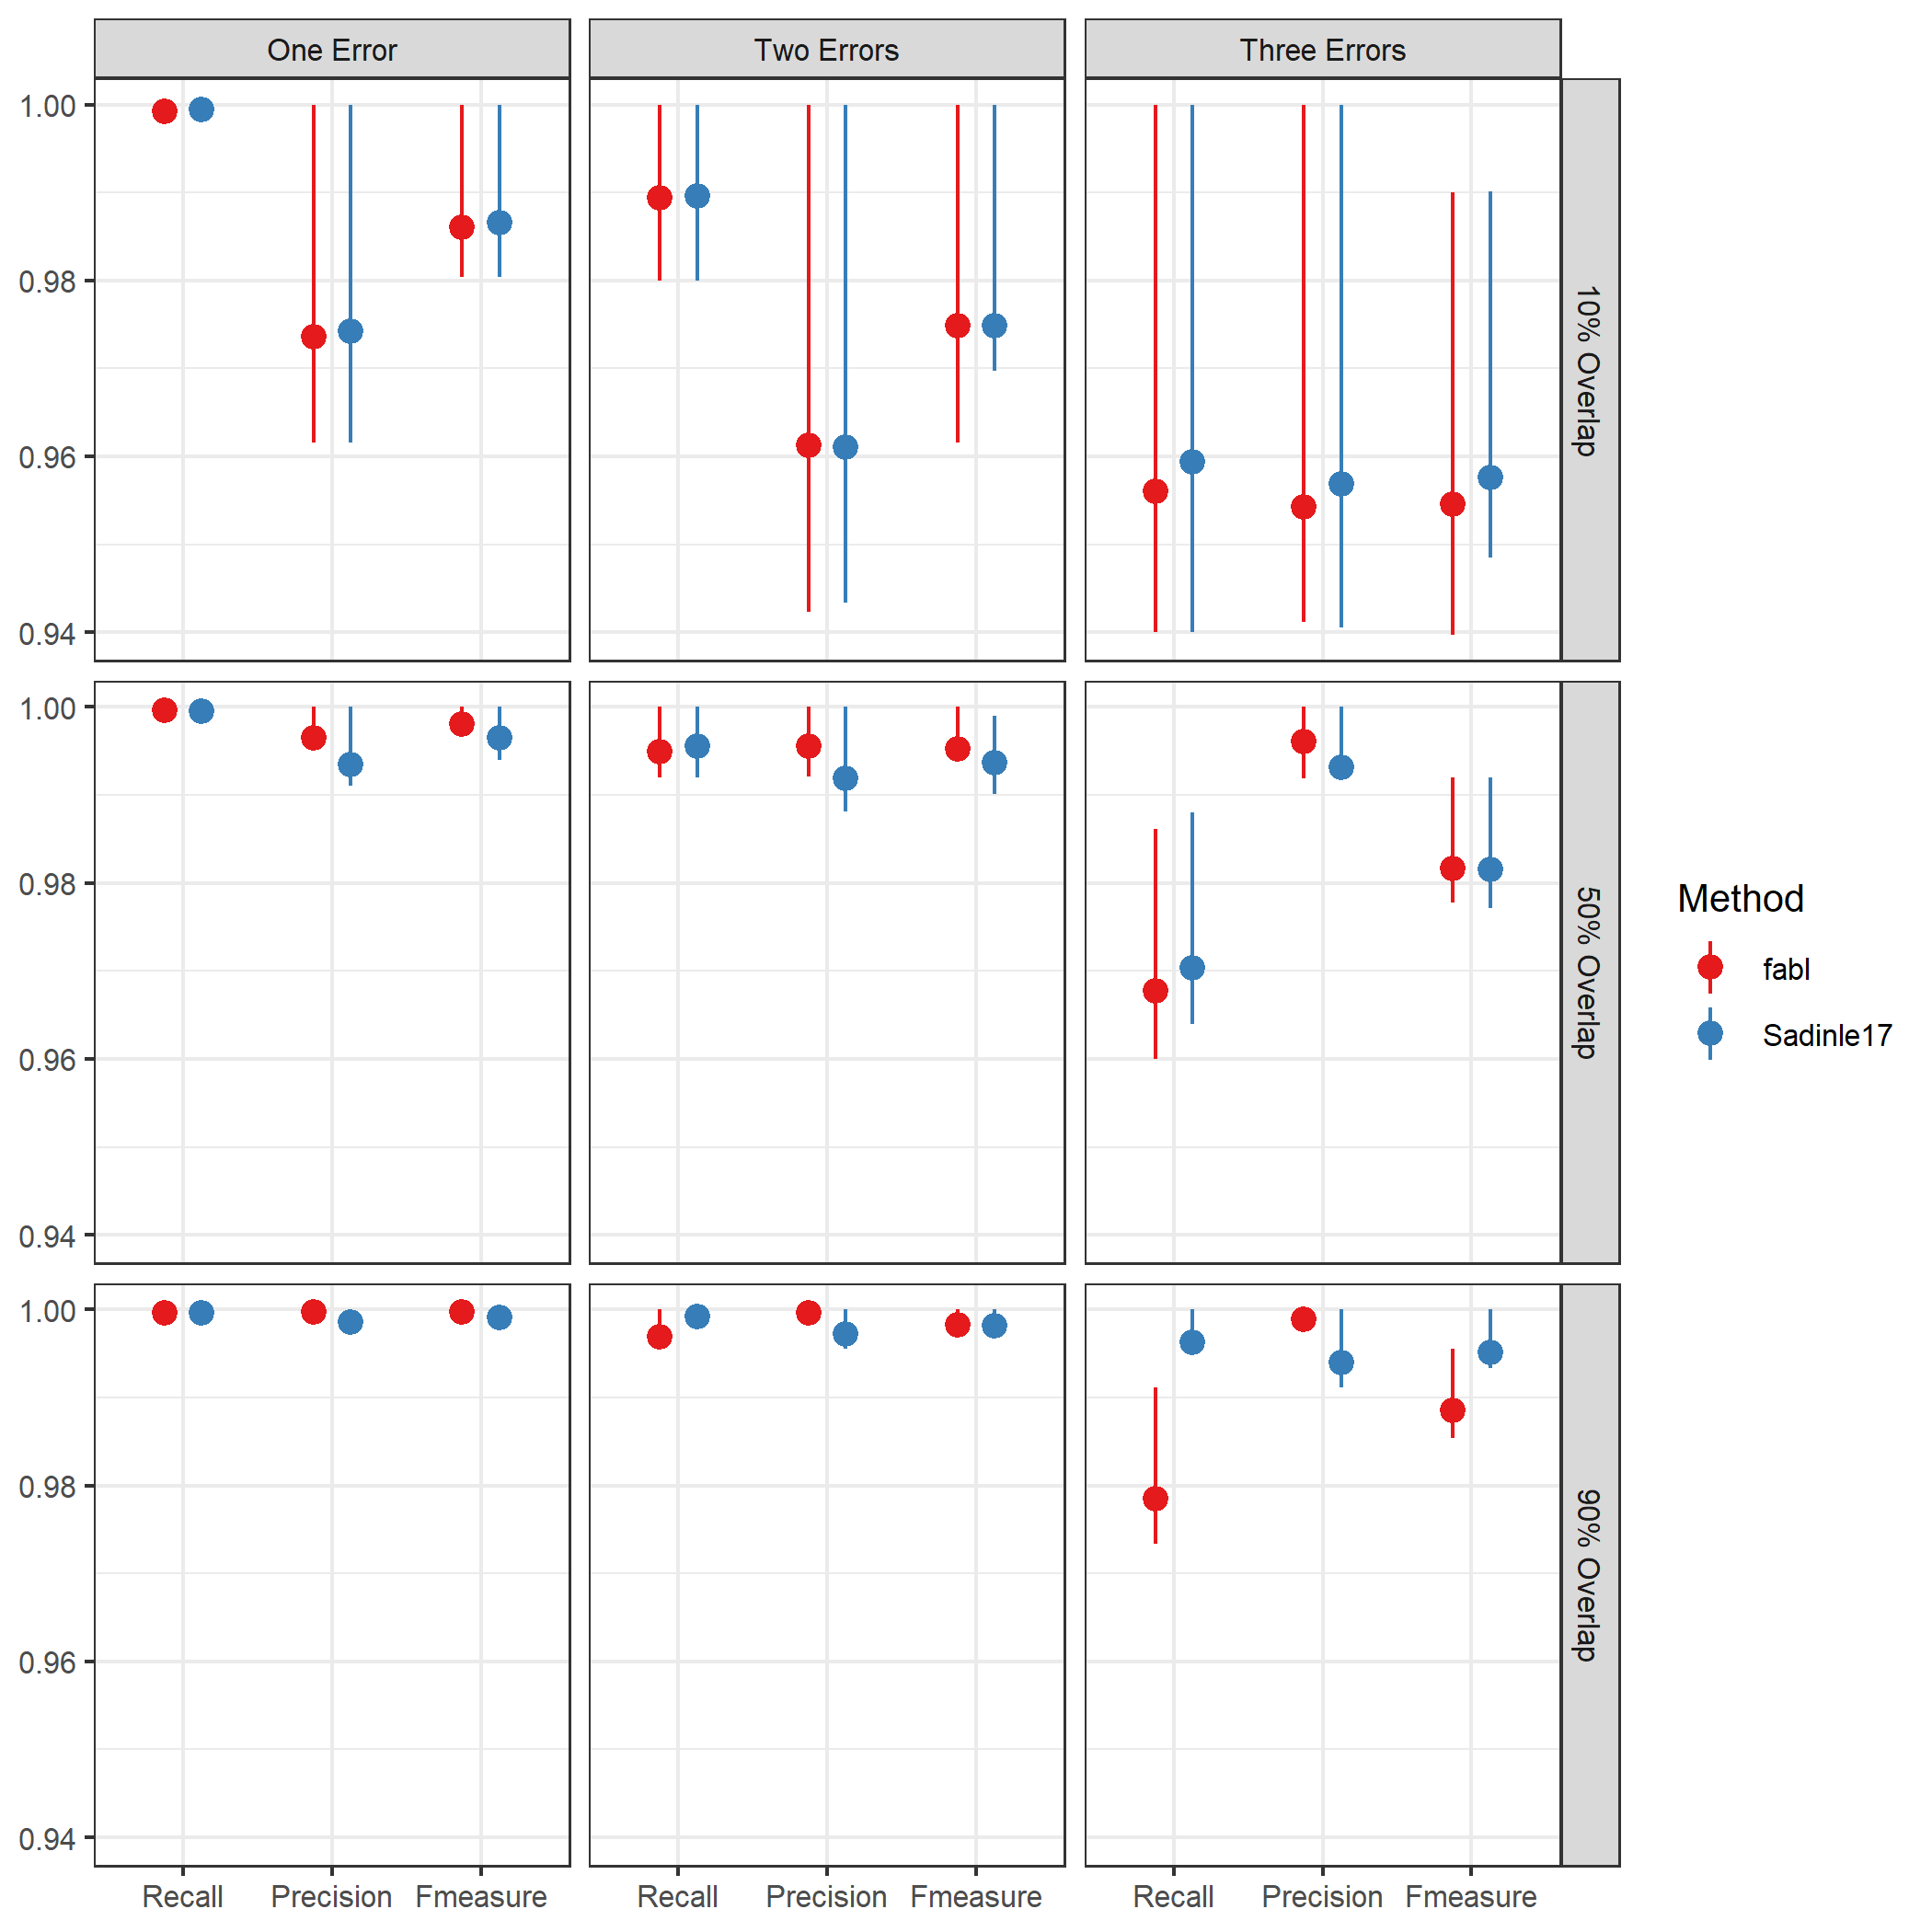
\includegraphics[width=0.6\textwidth]{../notes/figures/sadinle_sim_plot} 
\caption{Posterior means and credible intervals for accuracy metrics under the replication of simulation study from Sadinle 2017. For each level of overlap and each level of error, we have 100 paired sets of 500 records.}
\label{fig:sadinle_simulation}
\end{center}
\end{figure}

%
%\begin{figure}[ht]
%	
%	{\centering 
%		
%		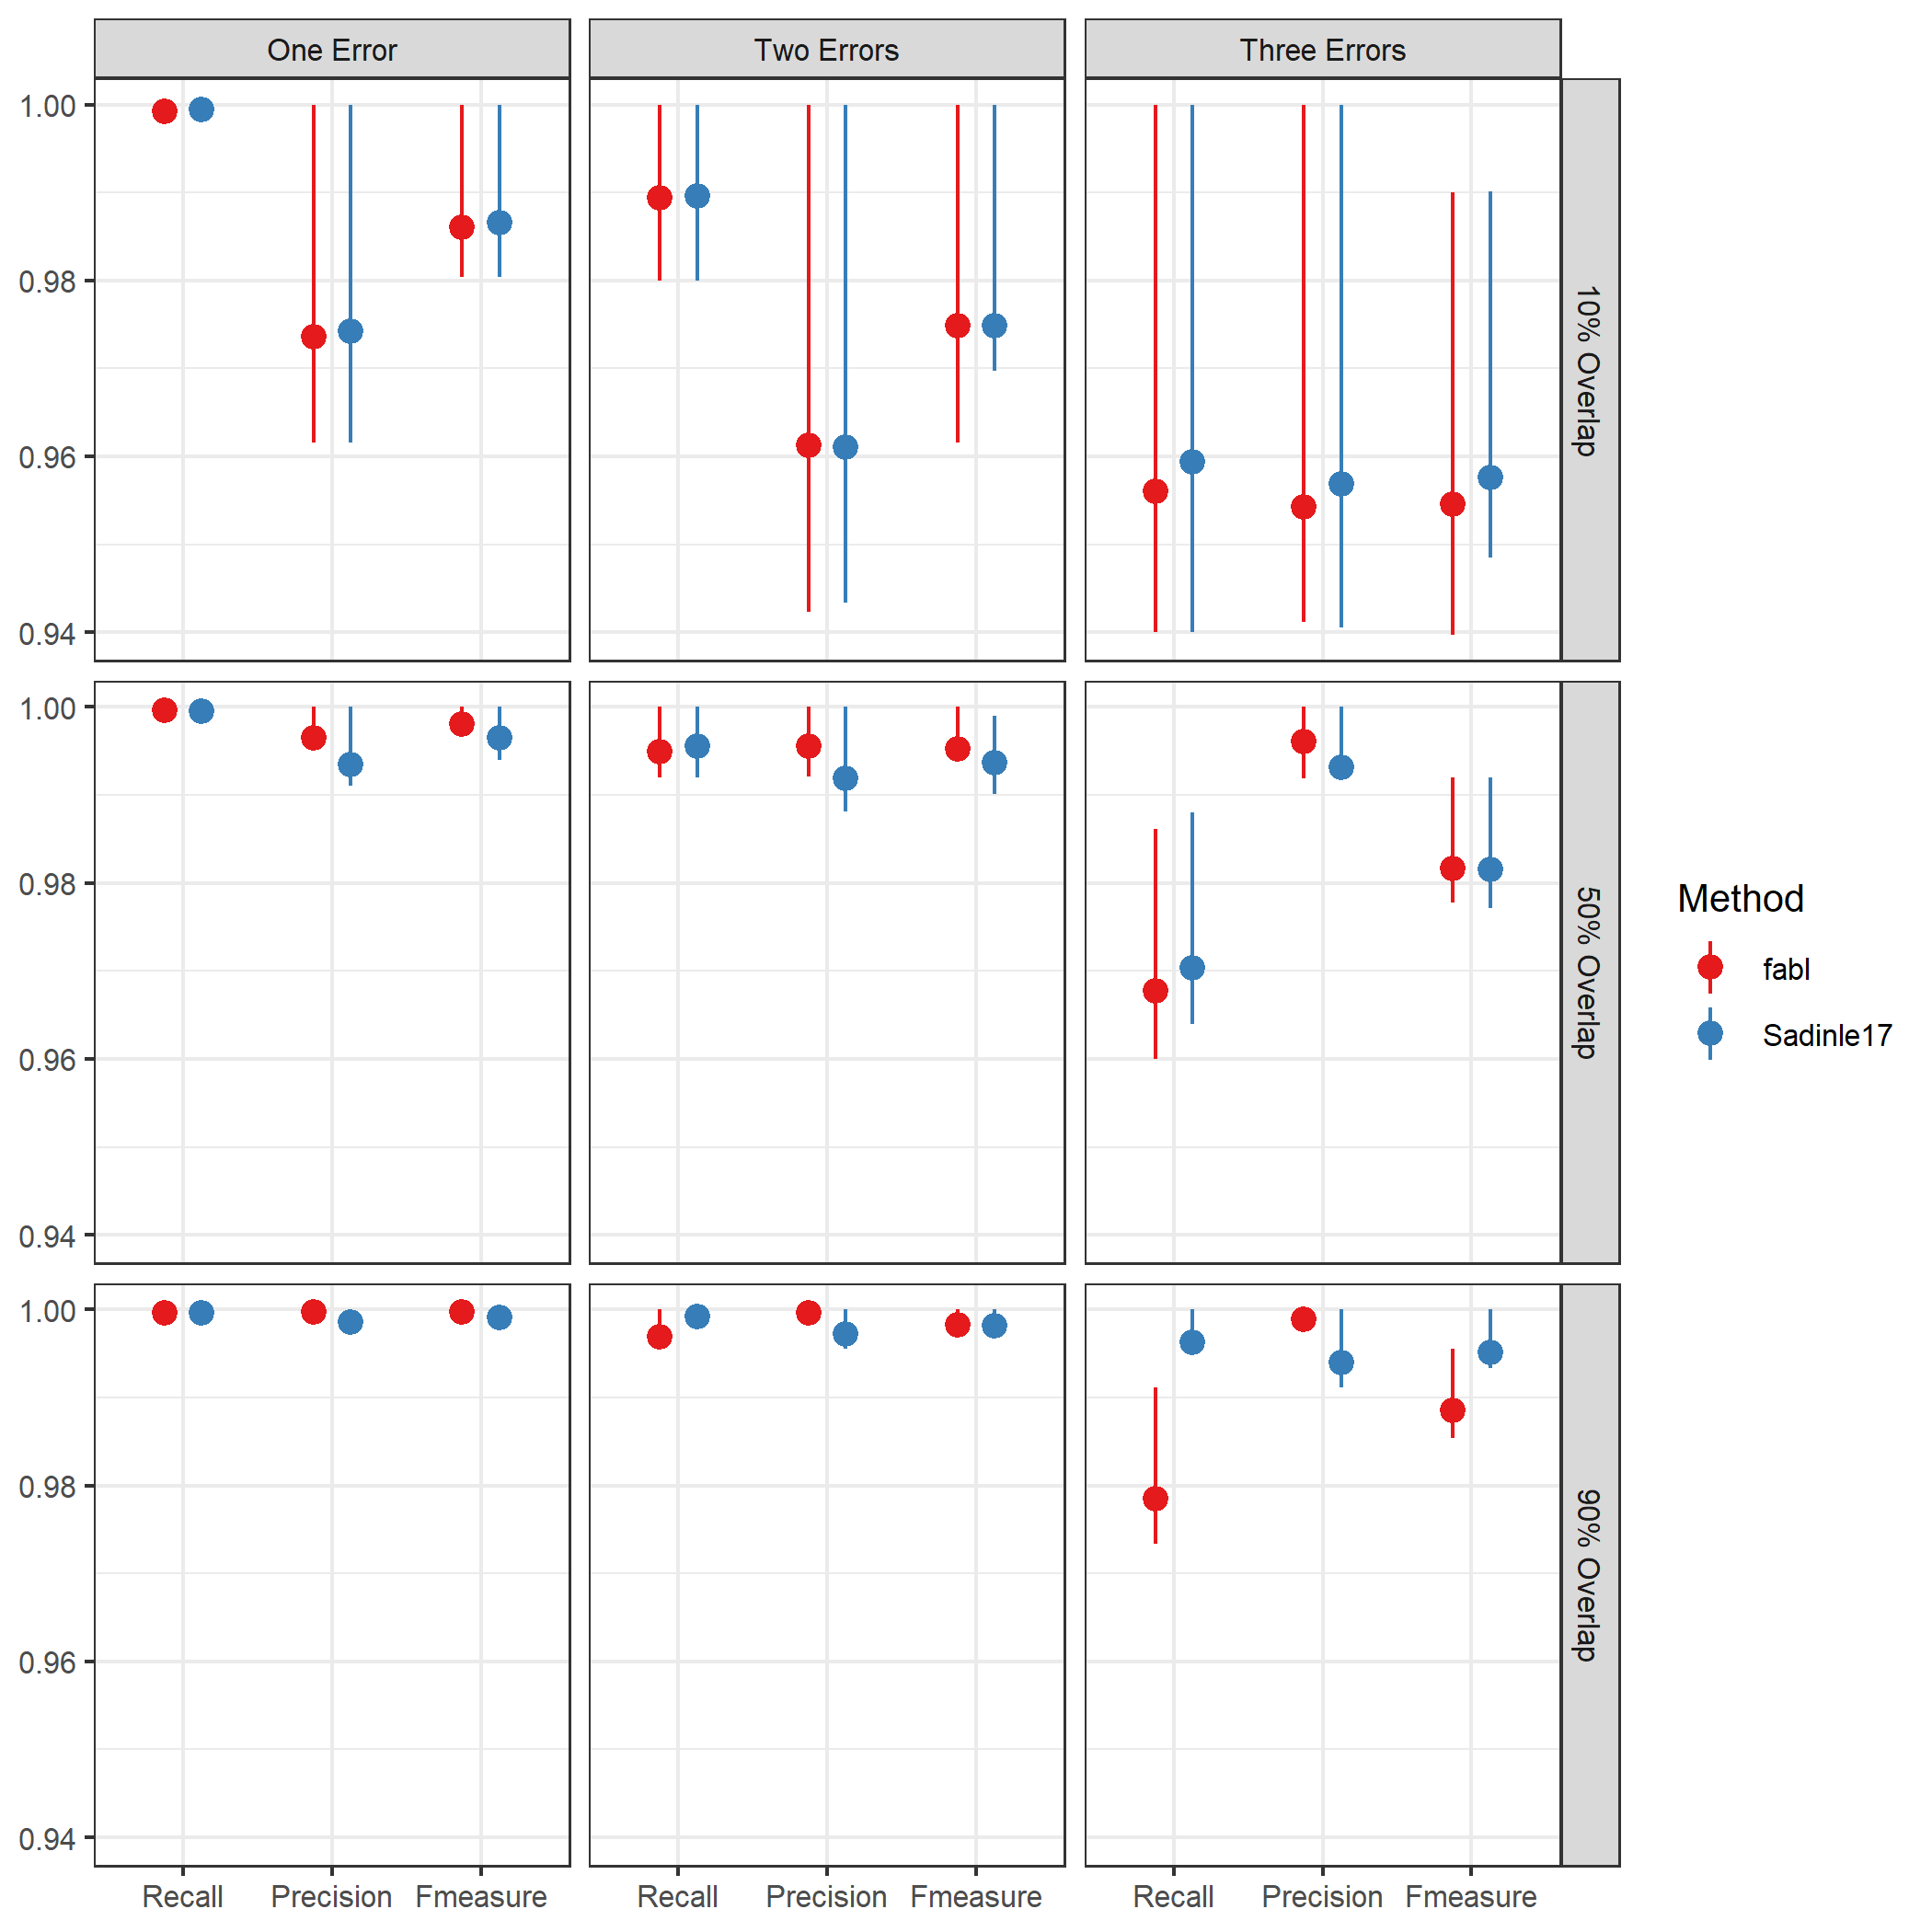
\includegraphics[width=0.6\textwidth]{../notes/figures/sadinle_sim_plot} 
%	}
%	
%	\caption{Posterior means and credible intervals for accuracy metrics under the replication of simulation study from Sadinle 2017. For each level of overlap and each level of error, we have 100 paired sets of 500 records.}\label{fig:sadinle_simulation}
%	
%\end{figure}

\hypertarget{speed}{%
	\subsection{Speed}\label{speed}}
	
\textcolor{red}{Brian: I have some general questions here. Are you using blocking for BRL to scale? Could you use the hashing proposal for BRL. It's important that the scale comparison be as fair as possible or there will be some pushback here. My suggestion around all this is to look at the computational complexity of both methods as it's hard to attack this.}	

To demonstrate speed, we generate comparison vectors from pre-specified
distributions so that we can easily increase the size of the linkage
problem. Distributions are meant to emulate the behavior of similarity
scores across first name, last name, and day, month. For example, $u^{\text{month, 1}} = P(\text{Records have same birth-month | Nonmatch}) = \frac{1}{12}$. For simplicity, we
consider only exact matching, so a vector (1, 0) corresponds to
agreement and (0, 1) to disagreement. We simulate these data for
different values of \(n_A\) and \(n_B\), and compare the run-time of
\texttt{fabl} against \texttt{BRL}. Note that the number of unique
patterns \(P\) is bounded above by \(2^5 = 32\), a bound which is
consistently attained in the larger simulations.

We see that at low data size, \texttt{BRL} outperforms, but that
\texttt{fabl} is significantly faster at handling larger data. In
particular, run-time for \texttt{BRL} seems to grow quadratically (or
linearly with the size of both \(A\) and \(B\)) while run-time for
\texttt{fabl} seems to grow linearly (in the size of \(B\)).

\begin{table}[t]
	\centering
	\begin{tabular}{rrr}
		\hline
		& m & u \\ 
		\hline
		fname & $\left(\frac{19}{20}, \frac{1}{20}\right)$ & $\left(\frac{1}{100}, \frac{99}{100}\right)$ \\ 
		lname & $\left(\frac{19}{20}, \frac{1}{20}\right)$ & $\left(\frac{1}{100}, \frac{99}{100}\right)$ \\ 
		day & $\left(\frac{19}{20}, \frac{1}{20}\right)$ & $\left(\frac{1}{30}, \frac{29}{30}\right)$ \\ 
		month & $\left(\frac{19}{20}, \frac{1}{20}\right)$ & $\left(\frac{1}{12}, \frac{11}{12}\right)$ \\ 
		year & $\left(\frac{19}{20}, \frac{1}{20}\right)$ & $\left(\frac{1}{12}, \frac{11}{12}\right)$ \\ 
		\hline
	\end{tabular}
\caption{Distributions used for $m$ and $u$ probabilties in simulation studies}\label{fig:distributions}
\end{table}


\begin{figure}[ht]
	
	{\centering 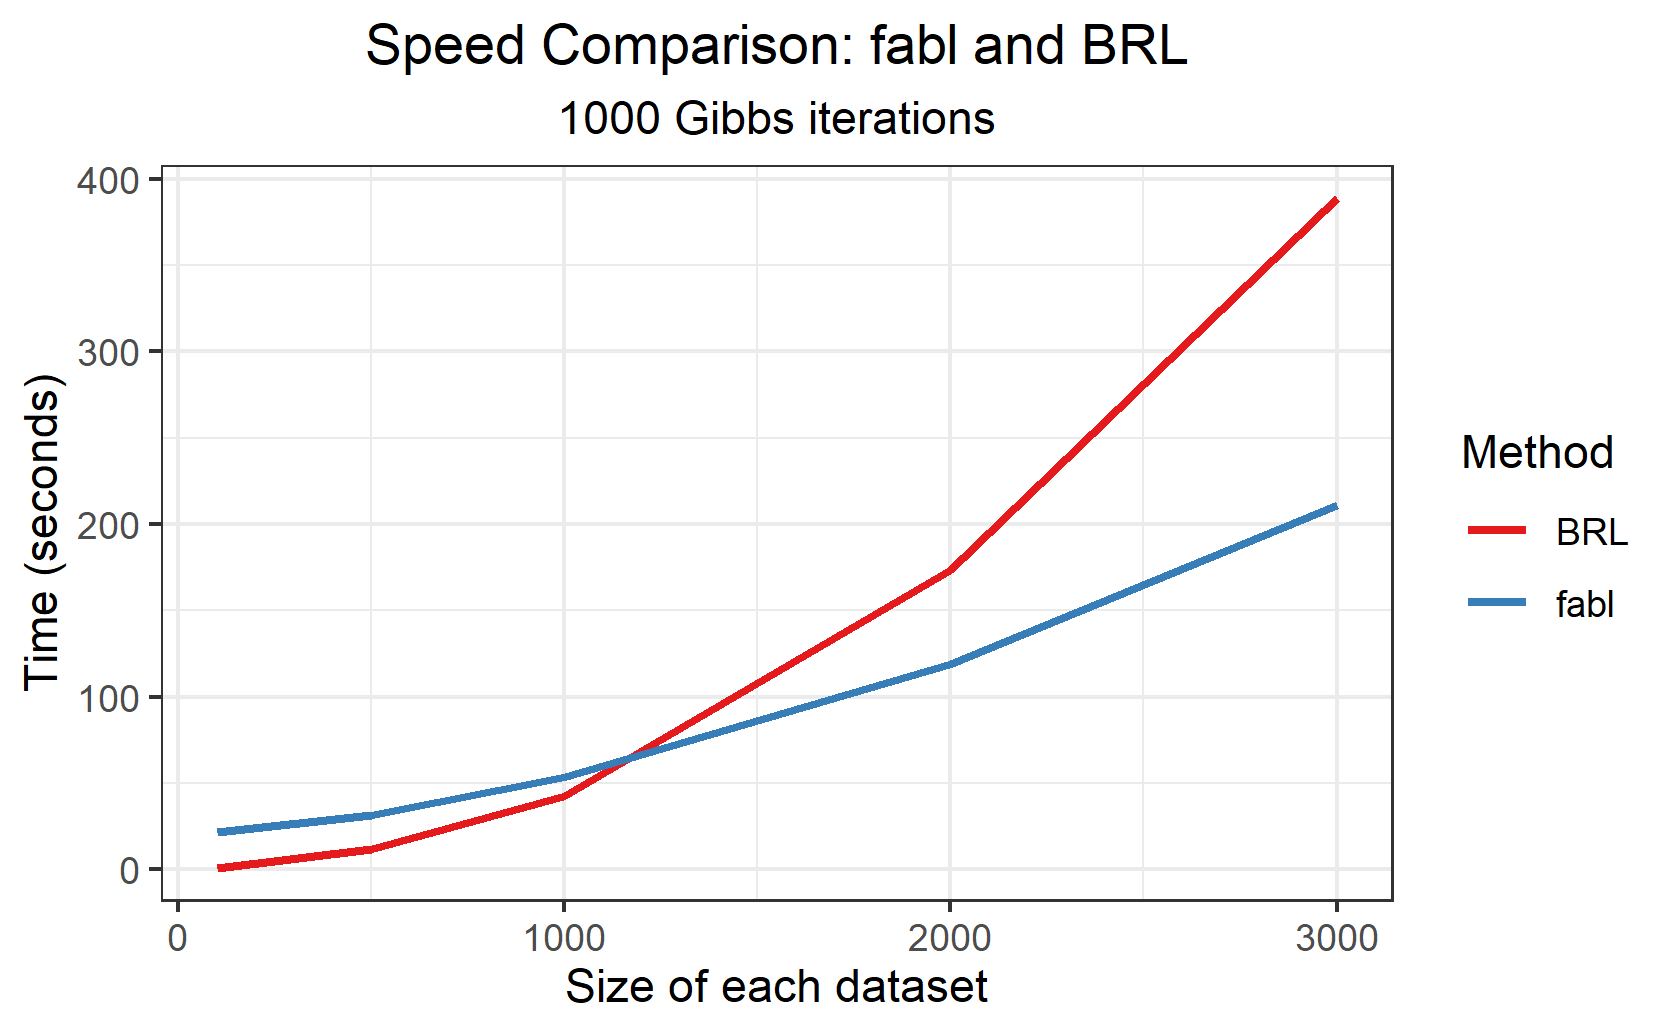
\includegraphics[width=0.6\textwidth]{../notes/figures/sadinle_speed_plot2} 
		
	}
	
	\caption{Run-time for BRL and fabl to run 1000 Gibbs iterations, including hashing step for fabl, for increasing values of both $n_A$ and $n_B$. We see near quadratic growth in runtime for BRL, and near linear growth for fabl.}\label{fig:speed1}
\end{figure}

The above discussion suggests that for fixed \(n_B\), computation time
should remain mostly constant with growing \(n_A\). Simulation study
suggests that this is true. In the plot below, fixing \(n_B = 500\), we
see linear growth for the run-time under \texttt{BRL} as \(n_A\)
increases, with much more static run-time under \texttt{fabl}. The
slight increases in run-time that we do see are due primarily to the
hashing step, which again can be run in parallel for large data.

\begin{figure}[t]
	
	{\centering 
\includegraphics[width=0.6\textwidth]{../notes/figures/speed_plot_fixed_nB} 
		
	}
	
	\caption{Run-time for BRL and fabl to run 1000 Gibbs iterations, including hashing step for fabl, with increasing $n_A$, and $n_B$ fixed at 500. We see linear growth in runtime for BRL, and near constant runtime for fabl.}\label{fig:speed2}
\end{figure}

We note here that \texttt{BRL} is coded in C, which makes for unfair
comparison against \texttt{fabl}, currently only built in R.
Additionally, although \texttt{fabl} is amenable to parallelization,
this simulation was run on a single core. Running \texttt{fabl} in C++
with paralellization for the hashing step and sampling the matching
status of the record pairs should lead to even more computational gains.

\hypertarget{scale}{%
	\subsection{Scaling to a Larger Simulation Study}\label{scale}}

% Assuming a 16GB personal machine, standard record linkage methods using all-to-all comparisons can only function on tasks where the matrix of comparison vectors $\Gamma$ is less than 8GB. In the context of the above simulation, each comparison vector contains four integers, collectively requiring 16 bytes of memory; assuming files of equal lengths, this means the largest linkage task possible is around $7000 \times 7000$. 

In this section, we investigate scaling to larger data sets using our proposed methodology. 
 
Specifically, we demonstrate how partitioning and hashing the data through \texttt{fabl} method allows us undertake significantly larger linkage tasks. We concatenate two sets of 40 simulated datasets from the original simulation studies of \cite{} to create two larger files, each of 20,000 records (40,000 records total). Working on one machine, we sequentially compare records across chunks, hash results, and then synthesize summary statistics for the entire simulation. Under standard Fellegi Sunter procedures, this would require 400,000,000 comparison vectors, each consisting for four integers, resulting a final comparison matrix about 6.4 GB in size. 
 
For simplicity, we partition one dataset into 20 smaller chunks, and leave the second dataset fully intact. We compare records, hash results, and then synthesize summary statistics for all 20 chunk comparisons. The resulting data object is now only 90 MB, about 1\% the size of the object required under the standard method. Executed sequentially, these comparisons and the Gibbs sampler take about one hour to run; using distributed computing. However, this could be sped up. 

Turning to evaluation metrics, this simulation achieved 96.5\% recall and 97.7\% precision, with an overall F-measure of 97.1\% F-measure. The reader will note that this slightly worse performance than witnessed in the smaller simulation studies; this is expected because it is naturally more difficult to link more files with the same amount of information. With more linkage fields \texttt{fabl} maintains the high accuracy seen above. \textcolor{red}{Brian: you should look to see if you fix these in the post-processing step as this would be interesting/important.}
 
 \textcolor{red}{How long does it take on the same machine to run BRL. Can you run this? This can close this section out!}
 
 

\section{Application to Civilian Casualties from the El Salvadoran Civil War}
\label{sex:case-studies}

In this section, we revisit an application to the El Salvadoran Civil War, where we estimate the number of documented identifiable deaths (DID). Though the data files used here are small, this study shows how the computational complexity of \texttt{fabl} depends on the number of unique agreement patterns, and how significant computational gains can be achieved by simplifying the construction of the comparison vectors. This case study also considers the ramifications of 
independently sampling $Z_j$ rather than strictly enforcing one-to-one matching as done by \texttt{BRL}. 

%The second case study is the National Long Term Care Survey (NLTCS), a much larger linkage tasks which \texttt{BRL} is unable to complete but which we complete with \texttt{fabl} with relative ease. 

\subsection{El Salvadoran Civil War}
\label{el_salvador}

The country of El Salvador was immersed in civil war from 1980 to 1991,
and throughout the time, several organizations attempted to document
casualties of the conflict. When estimating the total number of
casualties, one cannot simply sum the numbers recorded by each
organization, as it is likely that the same individuals are recorded in
multiple casualty lists. Thanks to the Human Rights Data Analysis Group (HRDAG), we utilize 
two different sources, namely,  El Rescate - Tutela
Regal (ERTL) and the Salvadoran Human Rights Commission (CDHES, by its
acronym in Spanish). The ERTL dataset consists of digitized reports that
had been published throughout the conflict. The CDHES dataset consists
of casualties that had been reported directly to the organization, and
later digitized.

\textcolor{red}{Beka: These data sets need more information regarding how the data sets were collected as this is quite important. See Sadinle (2017) and references for info). }

There are several challenges with working with such data. Firstly, both
datasets have been automatically digitized, which inherently leads to
some degree of typographical error. Secondly, the CDHES records are all
second hand accounts reported by individuals, which can result in
additional errors. Lastly, the only fields recorded are given name, last
name, date of death, and place of death; it is relatively common for a
parent and child to share the same given name, resulting in
indistinguishable records for two different individuals. This last point
nearly breaks the earlier mentioned assumption that there are no
duplicates within files, and reveals a key difference between
\texttt{BRL} and our proposed method.

In this paper, we utilize records that have non-missing entries for given and last name, which results 
in \(n_1 = 4420\) files in CHDES and \(n_2 = 1323\) files
in ERTL. We standardized names to account for common misspellings
in the Spanish language. The string distance used is a modified Levenstein
distance to account for the fact that second names are often omitted.
Place of birth is recorded by municipality and department within that
municipality; however, since department was missing in 95\% of records
in CHDES and 80\% of records in ERTL, this was excluded from our analyses. 
Thus, we conduct record linkage using given name, last name,
municipality, and day, month, and year of death. We again use flat
priors for the \(\mathbf{m}\) and \(\mathbf{u}\) parameters. To our knowledge, we have followed the same guidelines/settings in \cite{sadinle_bayesian_2017}.

To mirror the original implementation of \cite{sadinle_bayesian_2017}, we construct the comparison
vectors using four levels of agreement for each field, according to the
thresholds provided in \textcolor{red}{Figure XX}. This took 422 seconds for our proposed
method, \texttt{fabl}, and 240 for \texttt{BRL}. However, we observed that posterior
distributions of several levels of the \(\mathbf{m}\) and \(\mathbf{u}\)
parameters were nearly identical, and that of the
\(4^5 \times 2 = 2048\) possible agreement patterns, only 1173 are
realized in the data. This leads us to believe that such high number of
agreement levels creates unnecessary distinctions in the data and makes
the comparison vectors less interpretable. 

Therefore we re-ran our analysis with fewer agreement levels for each field \textcolor{red}{(see Figure XX)}, and
obtained analogous results. With 216 possible agreement patterns, 159
were realized in the data, and our proposed method, \texttt{fabl} became was faster,
finishing in 124 seconds. Meanwhile \texttt{BRL} took 239 seconds,
relatively unchanged from the first implementation. This demonstrates
the way that the computational complexity of our method depends on the
number of unique agreement patterns, and how significant computational
gains can be made by simplifying the construction of the comparison
vectors. The estimates of the \(\mathbf{m}\) parameters under each method are very similar, as shown in
Figure~\ref{fig:m-and-u}.

\begin{figure}[htbp]
\begin{center}
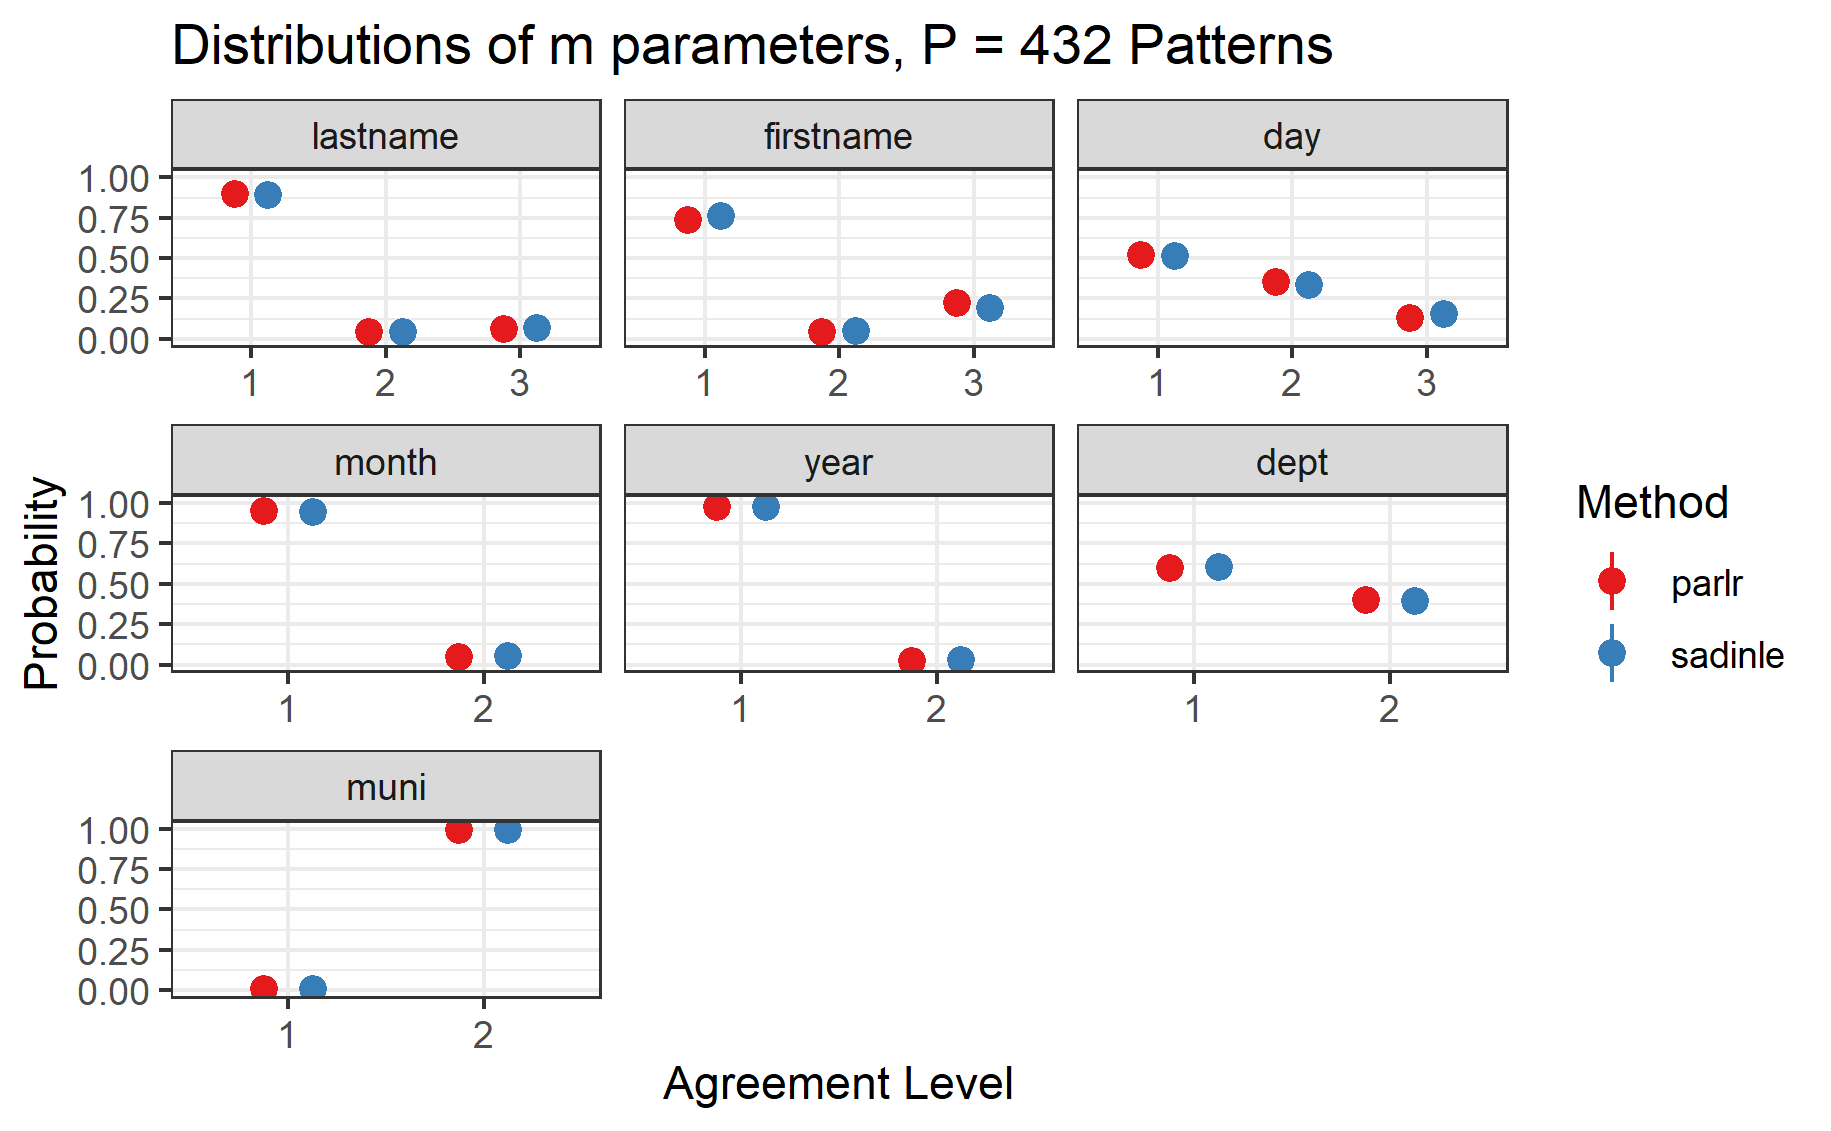
\includegraphics[width=0.6\textwidth]{../notes/figures/el_salvador/m_posterior_smallP} 
\caption{Posterior estimates of m parameters with 95\% credible intervals}\label{fig:m-and-u}
\label{fig:m-and-u}
\end{center}
\end{figure}



\paragraph{Violations of One-to-One Matching} 

In this section, we investigate violations of one-to-one matching of our method as compared to \texttt{BRL}.


Figure~\ref{fig:overlap-plot} shows the posterior distribution for \(D\), the number of
duplicates found in both databases for both \texttt{fabl} and \texttt{BRL}. We
see that \texttt{fabl} consistently overmatches within each Gibbs
iteration when compared to \texttt{BRL}, which is to be expected because
\texttt{BRL} explicitly prevents matches that violate one-to-one
matching throughout the entire sampler. Most of such matchings are due
to the randomness in the sampling procedure, and they occur sporadically
throughout the sampler in such a way that does not measurably influence
the eventual Bayes estimate.

\begin{figure}[htbp]
\begin{center}
 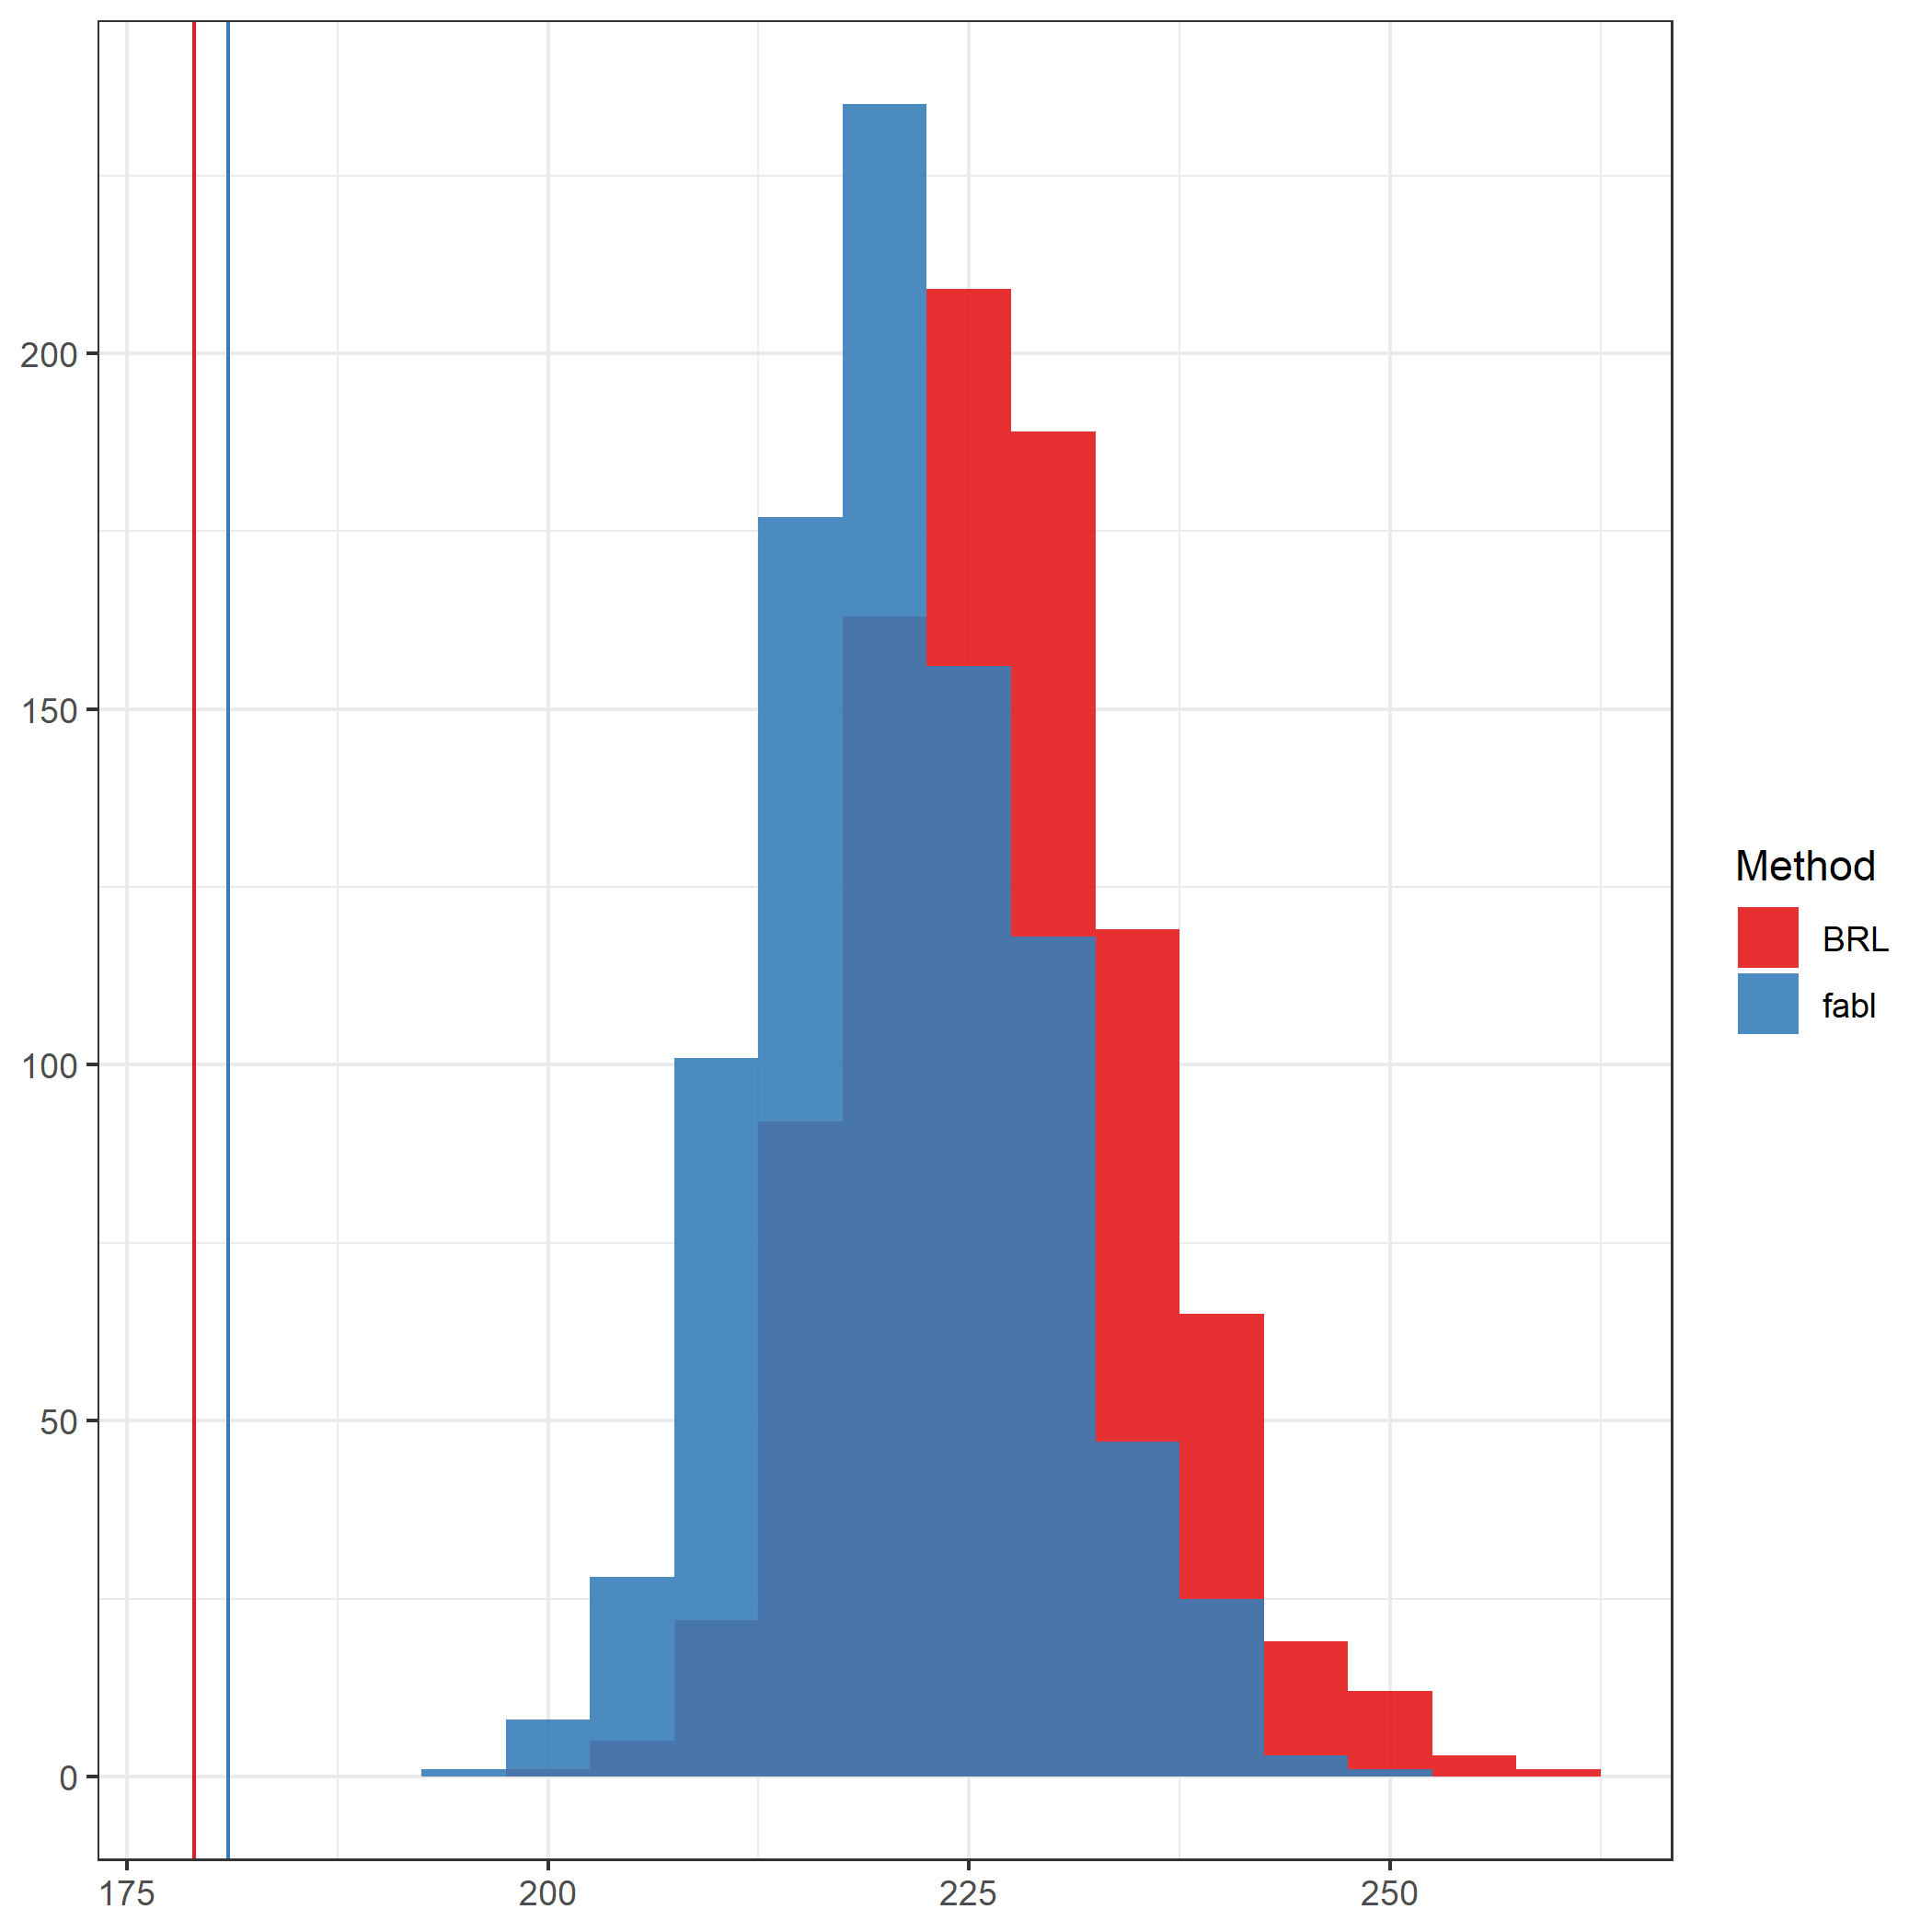
\includegraphics[width=0.6\textwidth]{../notes/figures/el_salvador/overlap_distribution_smallP_bayes} 
\caption{Posterior distribution of overlap across the two files. The solid lines show the Bayes estimate for the amount of overlap, and the dashed line is the Bayes estimate under fabl before resolving violations of one-to-one matching}
\label{fig:overlap-plot}
\end{center}
\end{figure}


%\begin{figure}[t]
%	
%	{\centering 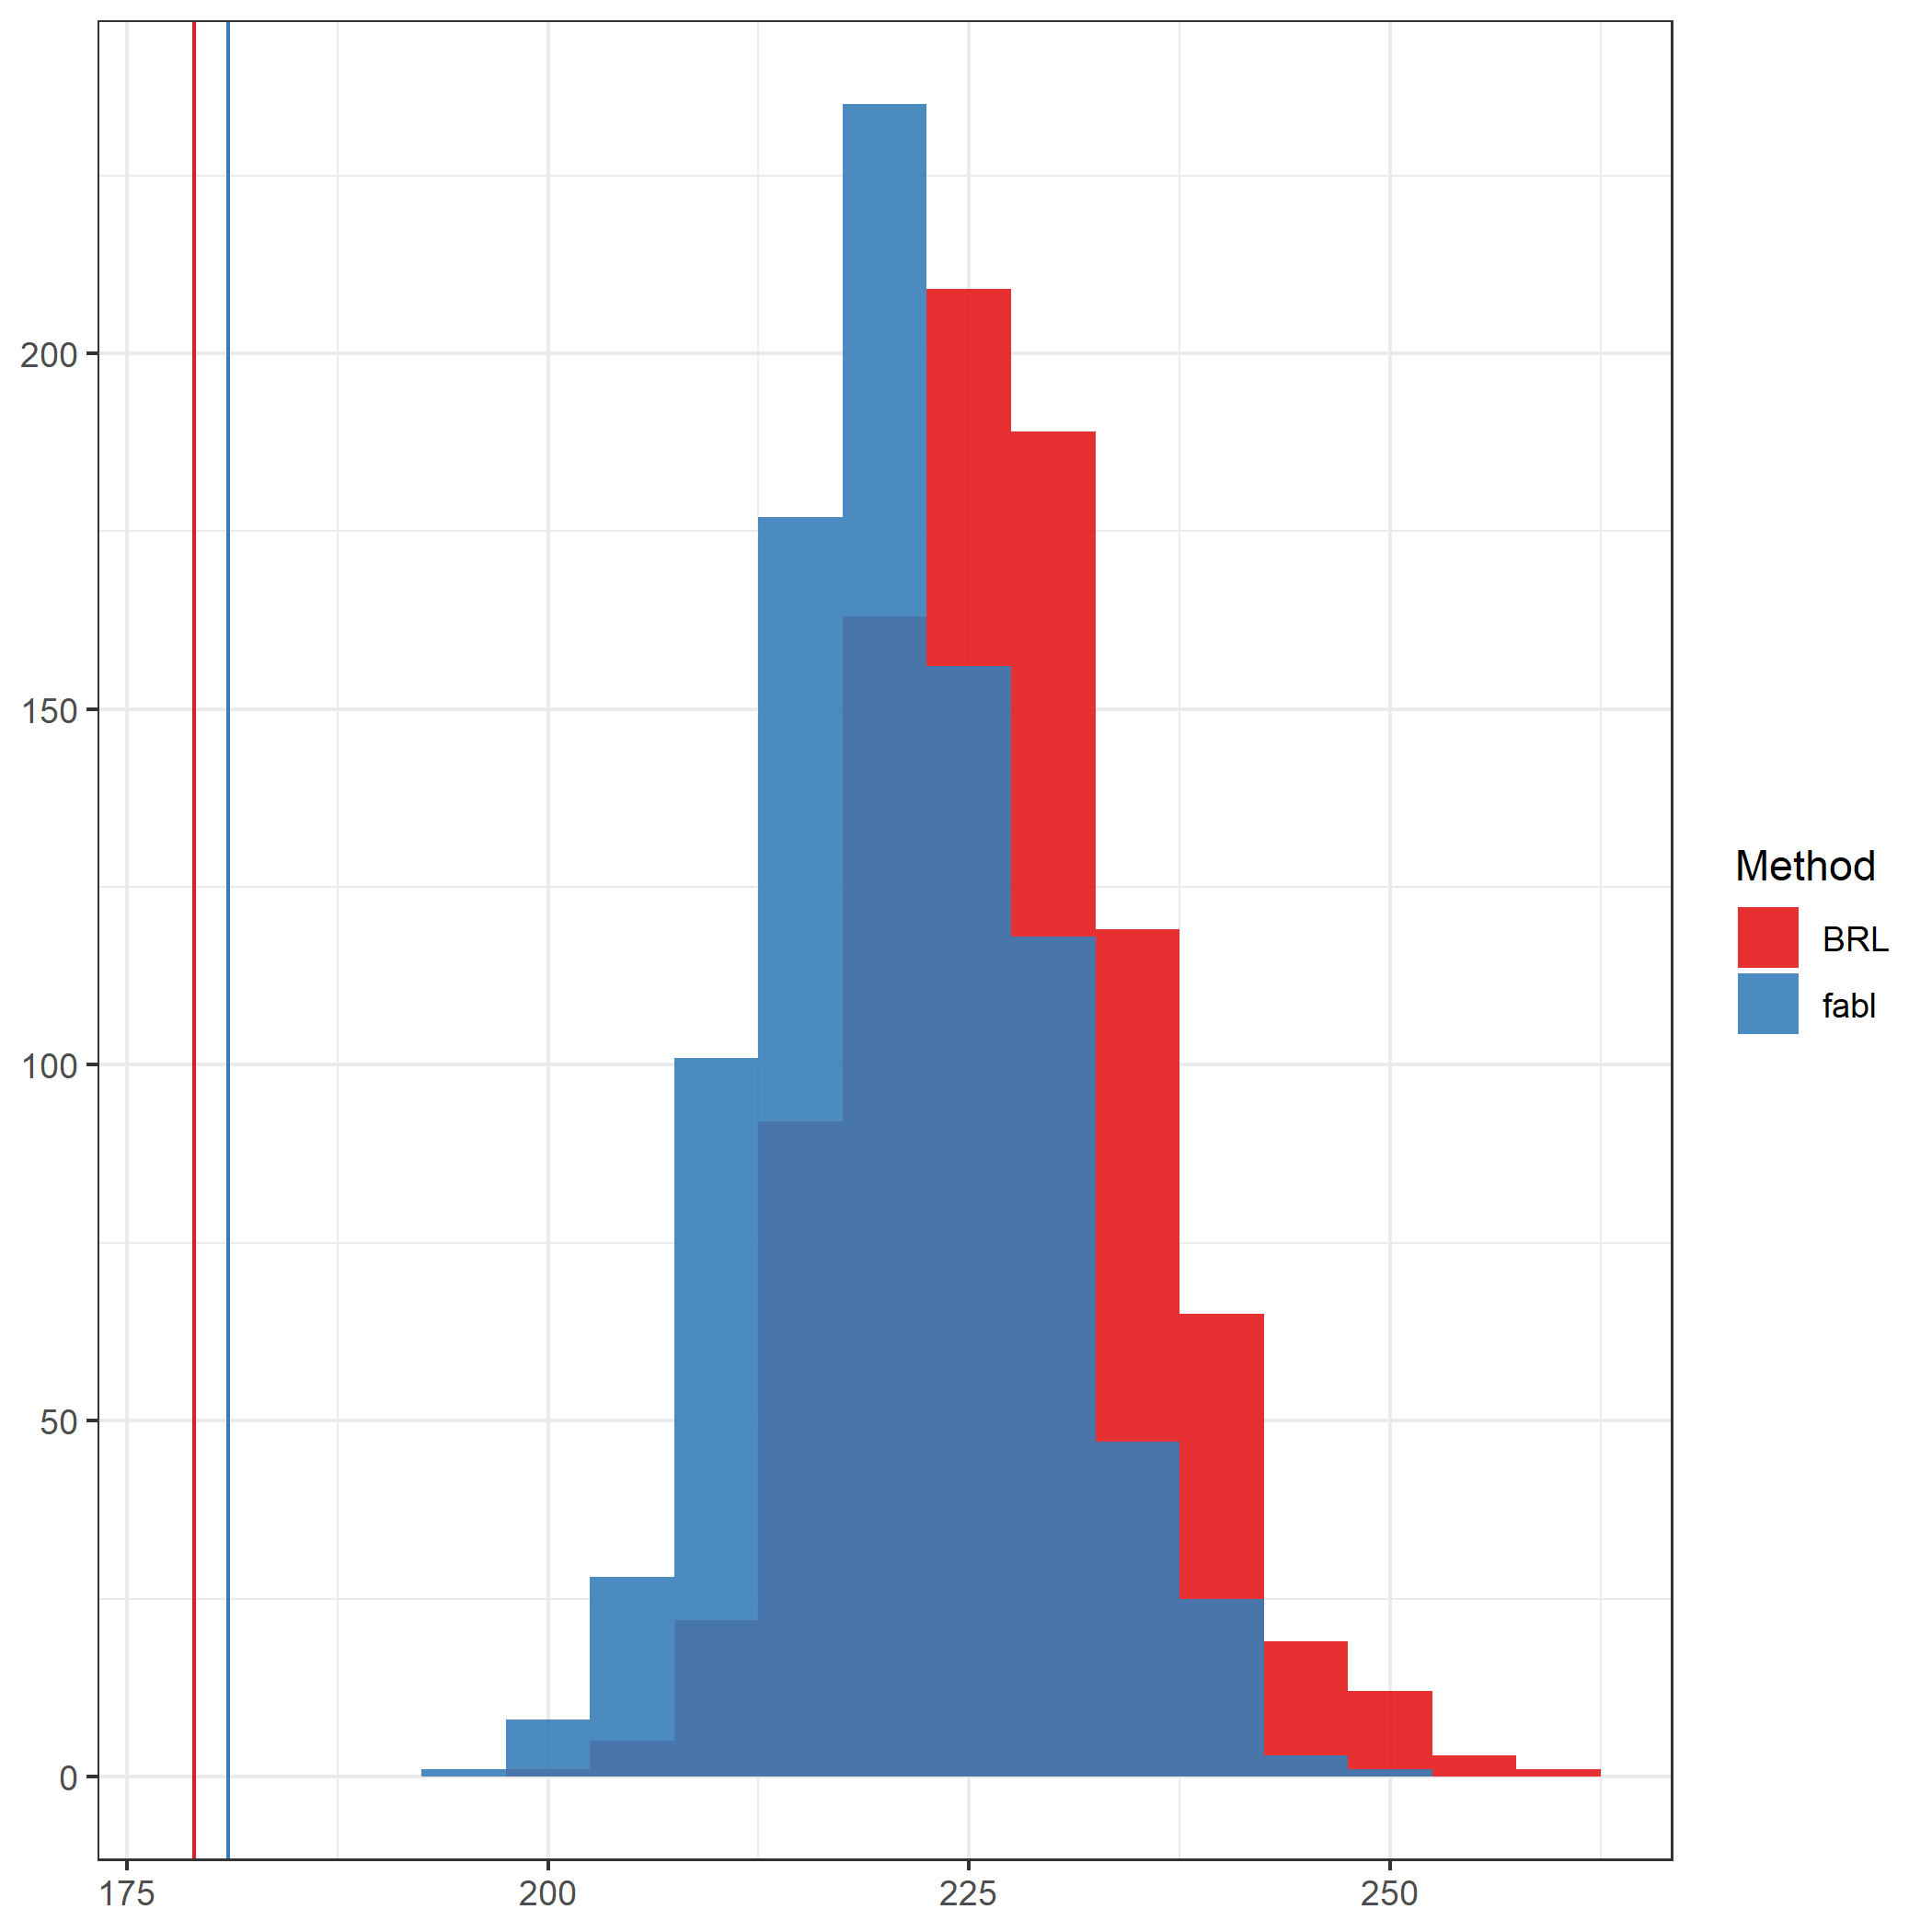
\includegraphics[width=0.6\textwidth]{../notes/figures/el_salvador/overlap_distribution_smallP_bayes} 
%		
%	}
%	
%	\caption{Posterior distribution of overlap across the two files. The solid lines show the Bayes estimate for the amount of overlap, and the dashed line is the Bayes estimate under fabl before resolving violations of one-to-one matching}\label{fig:overlap-plot}
%\end{figure}

Overall, both methods present similar results. \texttt{fabl} yields
an initial Bayes estimate of total 195 DID. After
resolving matches that violated one-to-one requirements,  we estimate 180 DID. 
\textcolor{red}{Can you report the posterior standard error for each one as we want uncertainty quantification.}


This is very close to the 181 DID found
by \texttt{BRL}. The main reason for this discrepancy is the difference
in how each model handles situations in which one file in \(\bm{X}_1\) has
multiple plausible matches in \(\bm{X}_2\).


%
%\begin{figure}[t]
%	
%	{\centering 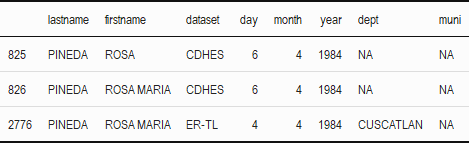
\includegraphics[width=0.6\textwidth]{../notes/figures/el_salvador/rosa_records} 
%		
%	}
%	
%	\caption{Example of linkage situation with multiple plausible matches}\label{fig:rosa-maria}
%\end{figure}



Figure~\ref{fig:rosa-maria} illustrates an example. Note these
records present a near violation of our assumption that there are no
duplications within files; we continue to assume that records 825 and
826 in ERTL correspond to different individuals, but their records are
nearly identical. In addition, using the modified Levenstein distance, the comparison vectors \(\gamma_{2776, 825}\) and
\(\gamma_{2776, 826}\) are exactly identical.

\begin{figure}[htbp]
\begin{center}
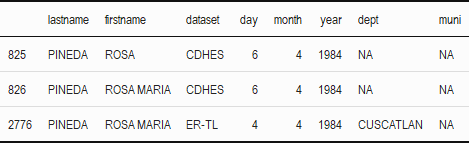
\includegraphics[width=0.6\textwidth]{../notes/figures/el_salvador/rosa_records} 
\caption{Example of linkage situation with multiple plausible matches}\label{fig:rosa-maria}
\end{center}
\end{figure}


Figure~\ref{fig:mixing-plot} shows the values that \(Z_{825}\) and \(Z_{826}\) take on
throughout the Gibbs sampler, and demonstrates how each method handles
this situation. Under \texttt{fabl}, both records in \(\bm{X}_2\) match to the
same record in \(\bm{X}_1\) throughout the Gibbs process, creating consistent
violations of one-to-one matching. Under \texttt{BRL}, the Gibbs process
creates one matching configuration and stays there for a while. However, if
one pair ``unmatches,'' then the other record has a chance to latch on.
Then, the Gibbs process is stuck with that matching status for a while,
resulting in a Gibbs process with poor mixing. In addition,
\texttt{fabl} allows the modeler to inspect records with multiple
plausible matches, and if they desire, to then choose the record pairing
with the highest posterior probability. \texttt{BRL} in contrast, in
strictly enforcing one-to-one matching throughout the sampler, can lead
to situations where none of the plausible matches reach the threshold to
be identified through the Bayes estimate. In short, we have pointed out why one may not wish to imbed this constraint in a model, and proposed a simple alternative that performs about the same as \texttt{BRL}, while scaling to much larger data sets. 

\begin{figure}[htbp]
\begin{center}
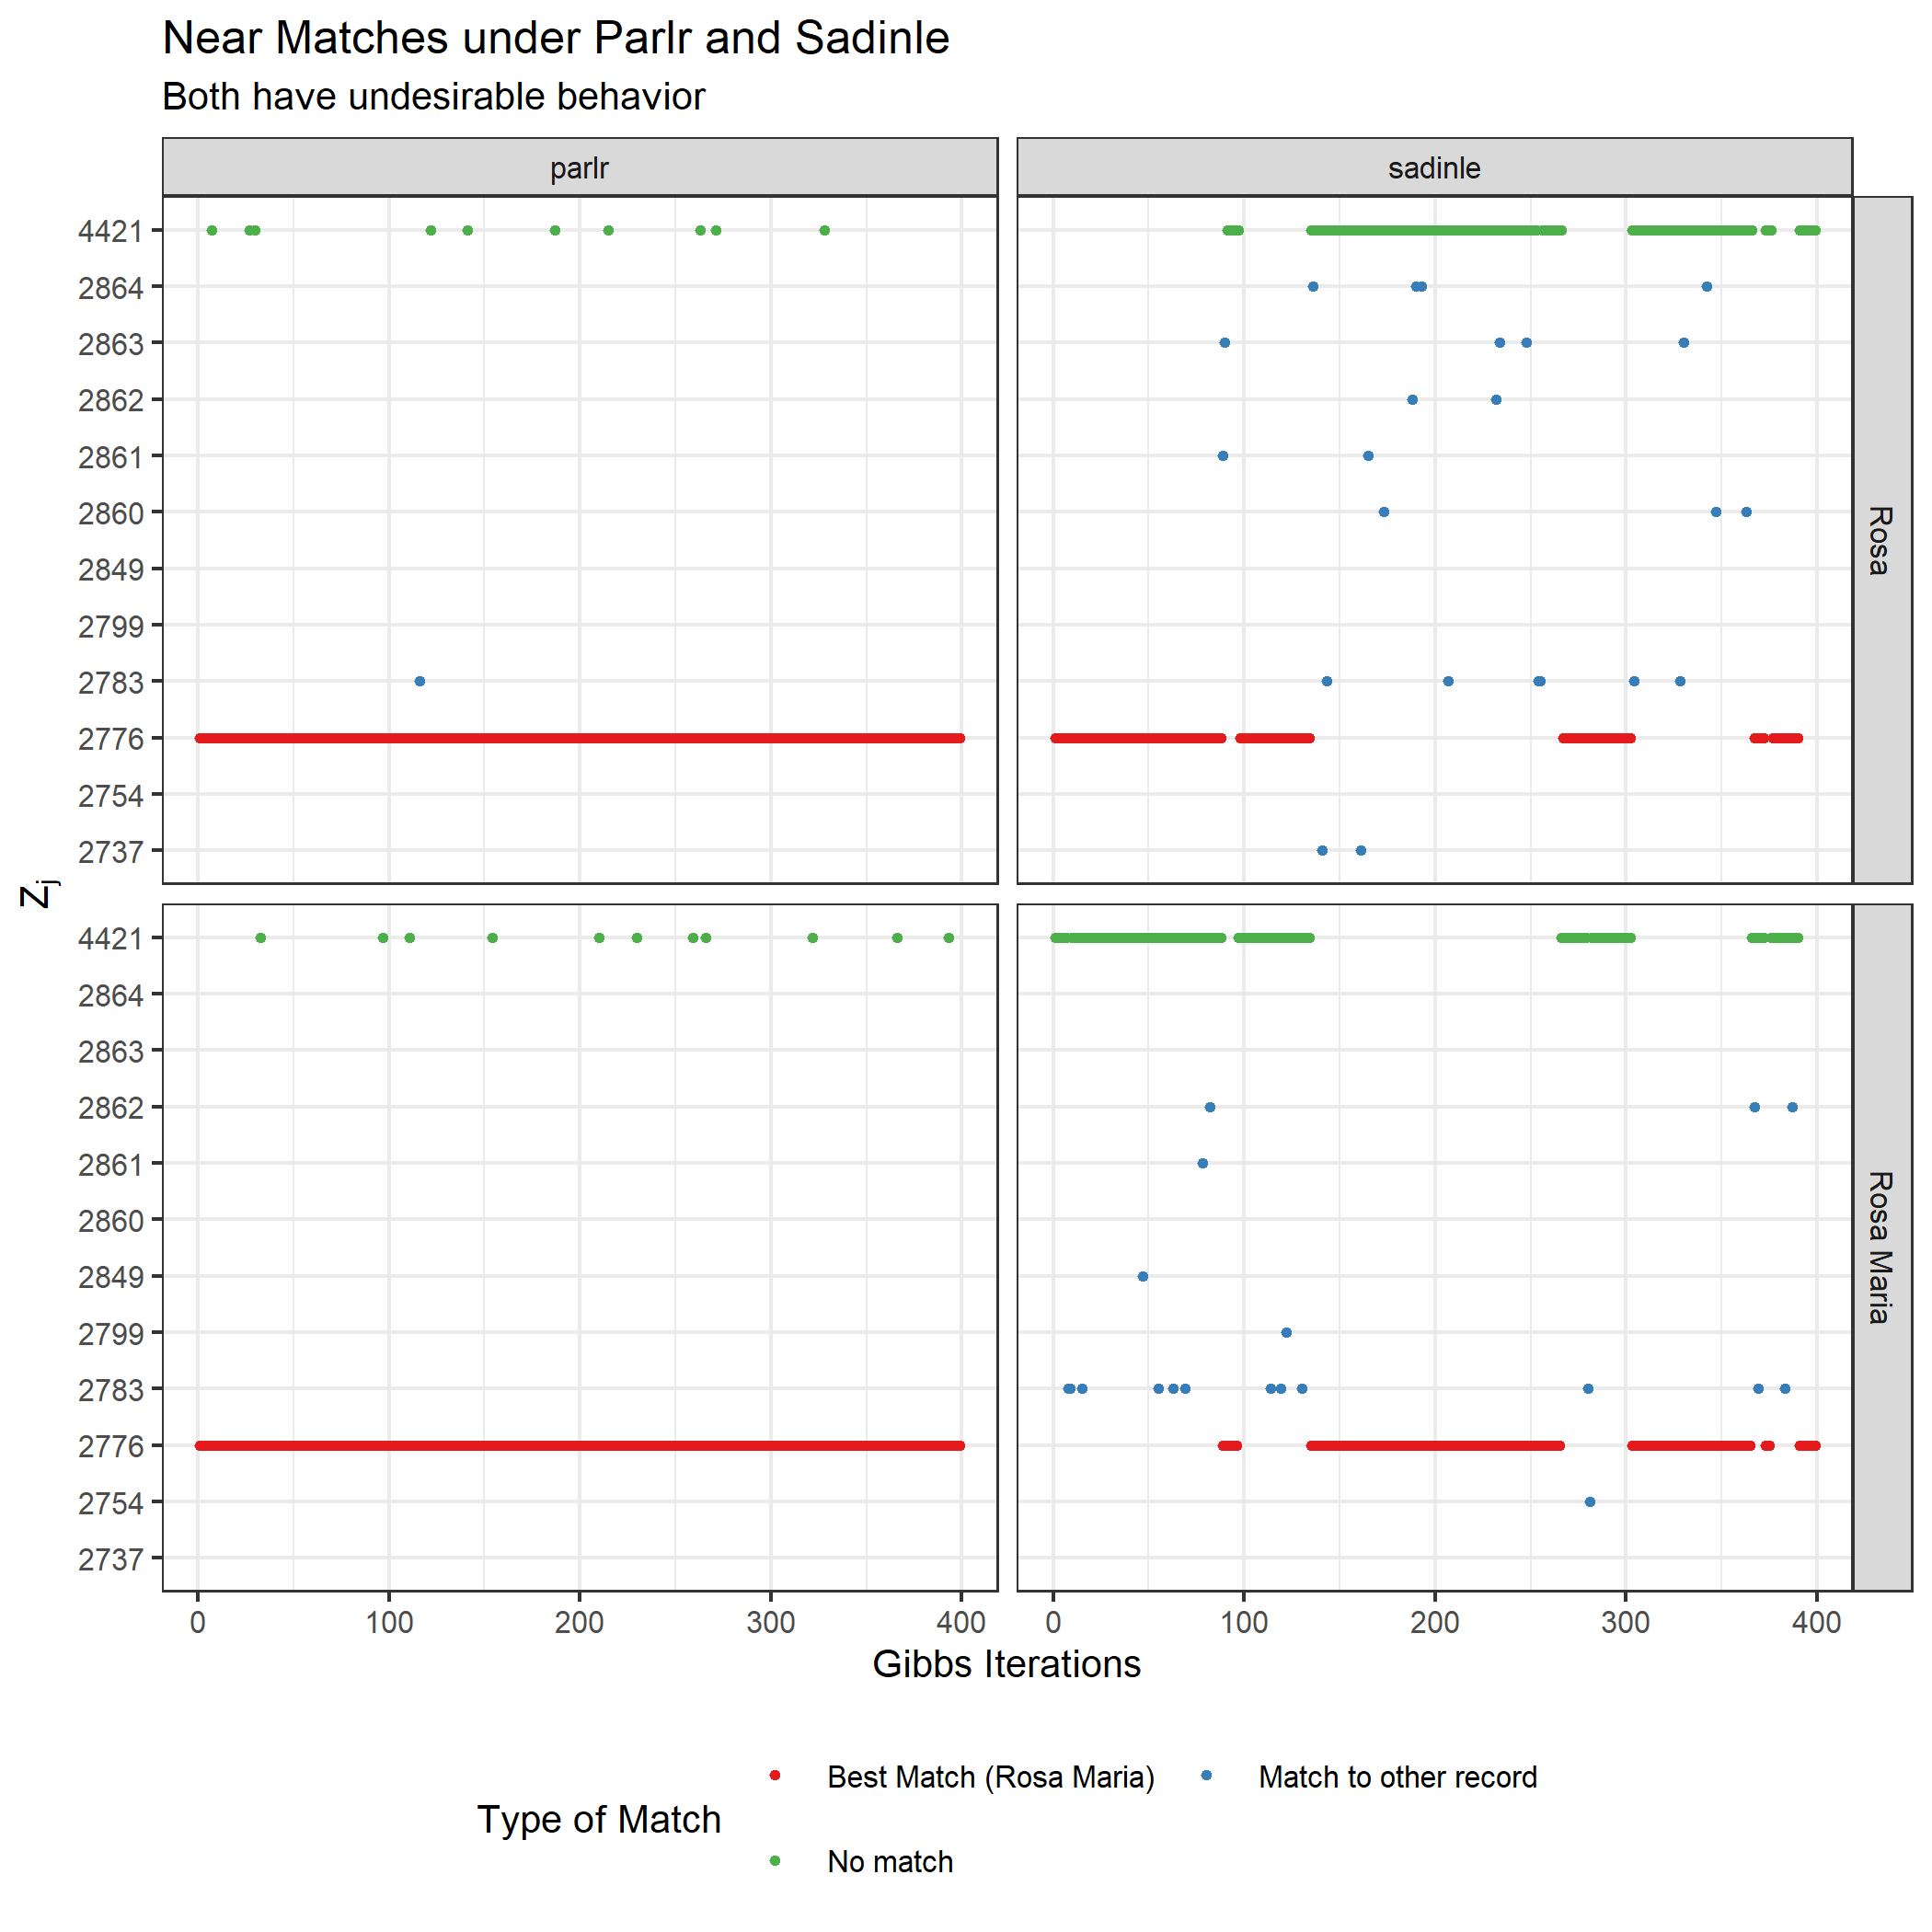
\includegraphics[width=0.6\textwidth]{../notes/figures/el_salvador/bad_mixing} 
\caption{Gibbs sampling in situation with multiple plausible matches.}\label{fig:mixing-plot}
\end{center}
\end{figure}


%\begin{figure}[t]
%	
%	{\centering 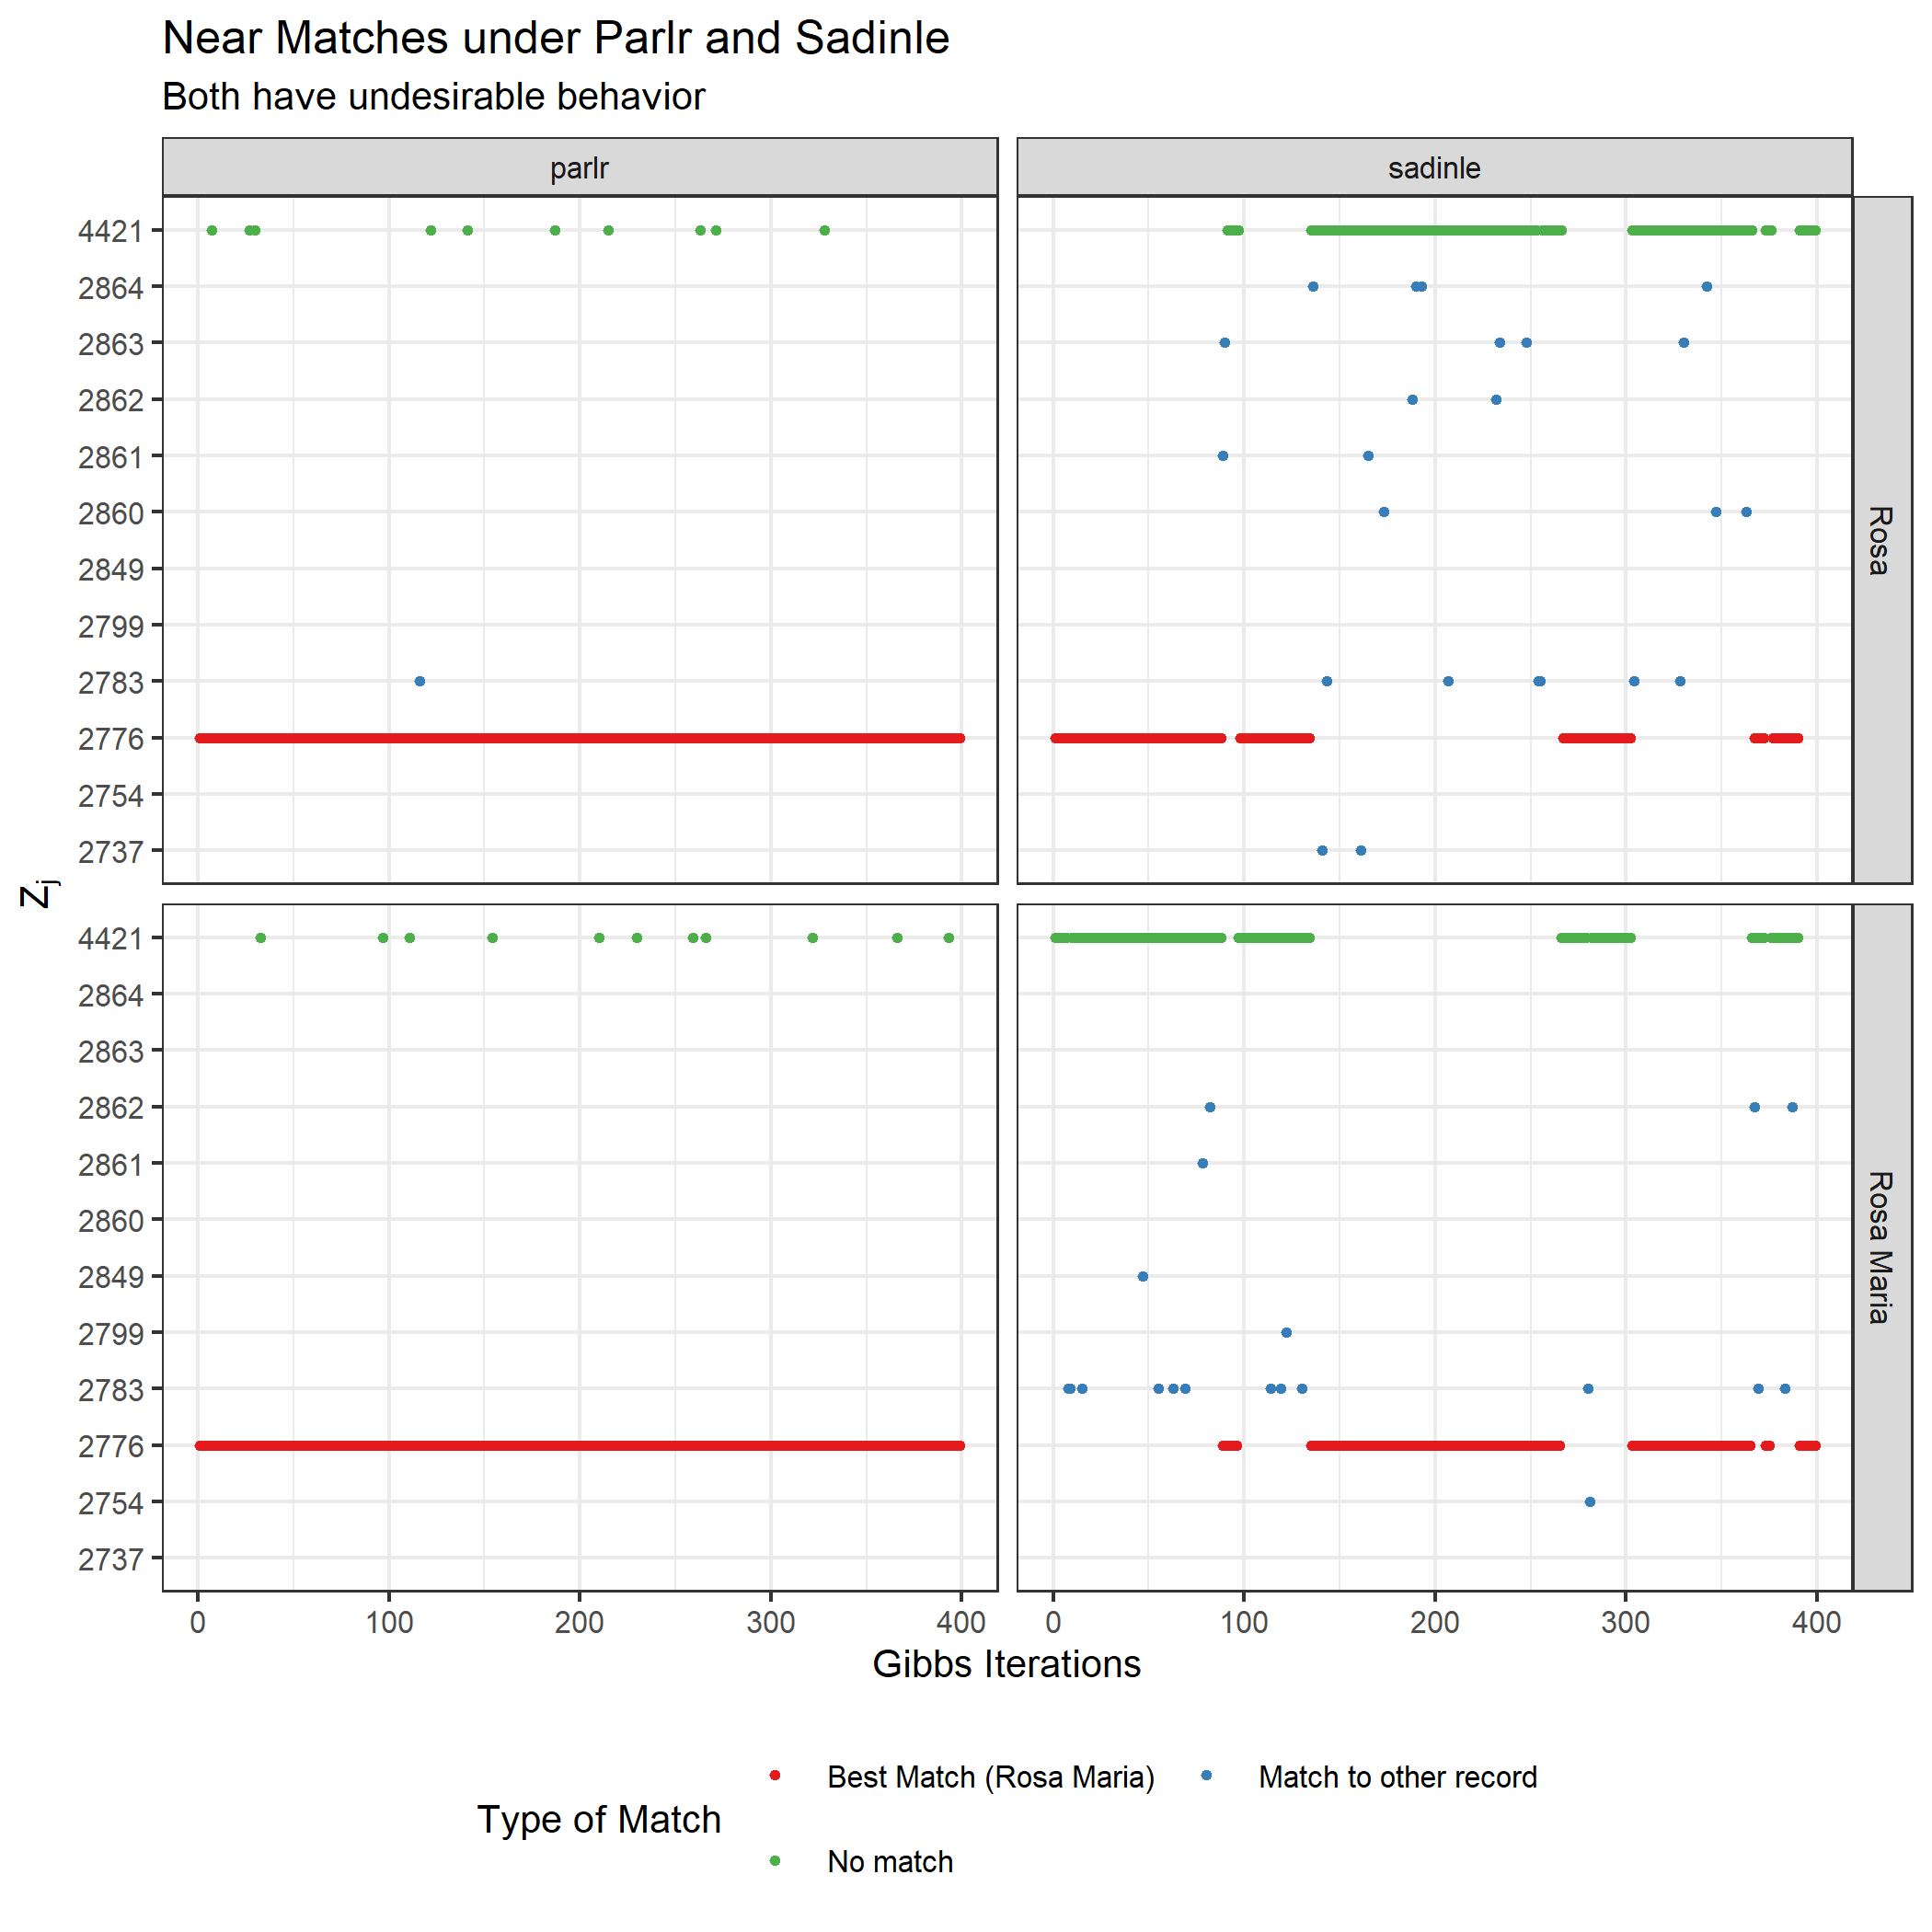
\includegraphics[width=0.6\textwidth]{../notes/figures/el_salvador/bad_mixing} 
%		
%	}
%	
%	\caption{Gibbs sampling in situation with multiple plausible matches.}\label{fig:mixing-plot}
%\end{figure}

%\subsection{National Long Term Care Survey}
%\label{nltcs} 
%
%The National Long Term Care Survey is a longitudinal study to track changes in health among Medicare recipients. It was conducted approximately every five years, and we concern ourselves here with linking records from years 1982 and 1989. The data only contains day, month, and year of birth, sex, state the individual lives in, and regional office. State and regional office have been anonymized, presented as numbers instead of their actual values. We construct the comparison vectors using only binary exact matching for each field, since there is no straightfoward way to incorporate partial matching in this context. The 1982 file contains $n_A = 20485$ records, 1989 file contains $n_B = 17466$ files, and the six linkage fields induces $2^6 = 64$ possible unique agreement patterns. We note that linkage quality is bound to be quite weak for many potential matches with such a large number of records and such limited identifying information.  
%
%With such large files, performing all-to-all comparisons under the original Fellegi-Sunter framework is infeasible. Indeed, this would require nearly 400 million comparison vectors, each containing 6 integer comparisons; the resulting data object would contain over 2 billion integers, and would require approximately 16 GBs of memory to hold. Instead, we take the partitioning approach reviewed in \ref{data-representation-hashing-and-storage}, and split each dataset into 10 smaller datasets. We use parallel computing on cluster service create the comparison vectors for each pair of data chunks, hash the results, and compress in size through storage efficient indexing. We then aggregate the results, creating a data object of just 87 MB, and proceed with the Gibbs Sampler. 
%
%Were a personal computer able to hold the 16 GB data object required by the direct approach, the Gibbs sampler under \texttt{BRL} would be tortuously slow, with computational complexity $O(n_A \times n_B \times F)$ where $n_A = 20485$. However, under \texttt{fabl} the sampler has complexity $O(P \times n_B \times F)$ where $P = 64$, so 1000 iterations of the Gibbs sampler are completed in just XX seconds. Posterior analysis yields an initial estimate of 9991 individuals linked across the the two datasets, and 8895 individuals linked once conflicts are resolved to ensure one-to-one matching. 
%
%Lastly, we comment on the significance of conducting this linkage without the use of deterministic blocking. With previous methods, one could link these two records by blocking on a certain field, and running separate Gibbs samplers on each of the separate blocks. This strategy drastically improves computation since it significantly reduces the number of comparison vectors that need to be formed and uses smaller data objects throughout the sampler. However, this computational savings comes at the cost of missing potential links, specifically in cases where the blocking variable is recorded in error. In this case, 62 of the matched pairs exhibit a disagreement in sex, 17 exhibit a disagreement in state, and 39 exhibit a disagreement in regional office. We have no way to verify that the matches found under \texttt{fabl} are indeed correct, so it is possible that matches found with such disagreements are false positives. Even if not, the modeler may conclude that, for example, 17 missed matches are a small price to pay to be able to block on state and run 50 smaller, independent linkage procedures. However, \texttt{fabl} allows the modeler to make this choice for themselves, rather than being forced to do so for computational reasons. Additionally, by running on the Gibbs sampler the entirety of both files, we achieve $m$ and $u$ parameters that are interpretale for the entire study, rather than separate parameters for each block. Although these $m$ and $u$'s are often regarded as nuisance parameters in the record linkage literature, \texttt{fabl} allows for study of these parameters that has been been possible before. 

\section{Discussion}
\label{discussion}

We have presented a method for Bayesian record linkage that is feasible
for large datasets. In particular, our hashing procedure and model
assumptions allow for a linkage procedure whose computational complexity
does not scale with the size of the larger dataset, making this method
particularly powerful in linking records when one datafile is
substantially smaller than the other.

In our case study, we included an exploration of how to conduct record
linkage when modeling assumptions are not met in practice. We explored
``one-to-many'' scenarios in which one record in \(A\) has multiple
plausible matches in \(B\), and showed how both \texttt{fabl} and
\texttt{BRL} demonstrated undesirable qualities. Other issues arise
under ``many-to-one'' scenarios, where one record in \(B\) has multiple
plausible matches in \(A\), and ``many-to-many'' scenarios in which
there is duplication both across and within datasets. Tuning
\texttt{fabl} for use in these scenarios is one potential avenue for
future work.

\bigskip

\section{Appendix}
\label{sec:appendix}

\begin{figure}[t]
	
	{\centering 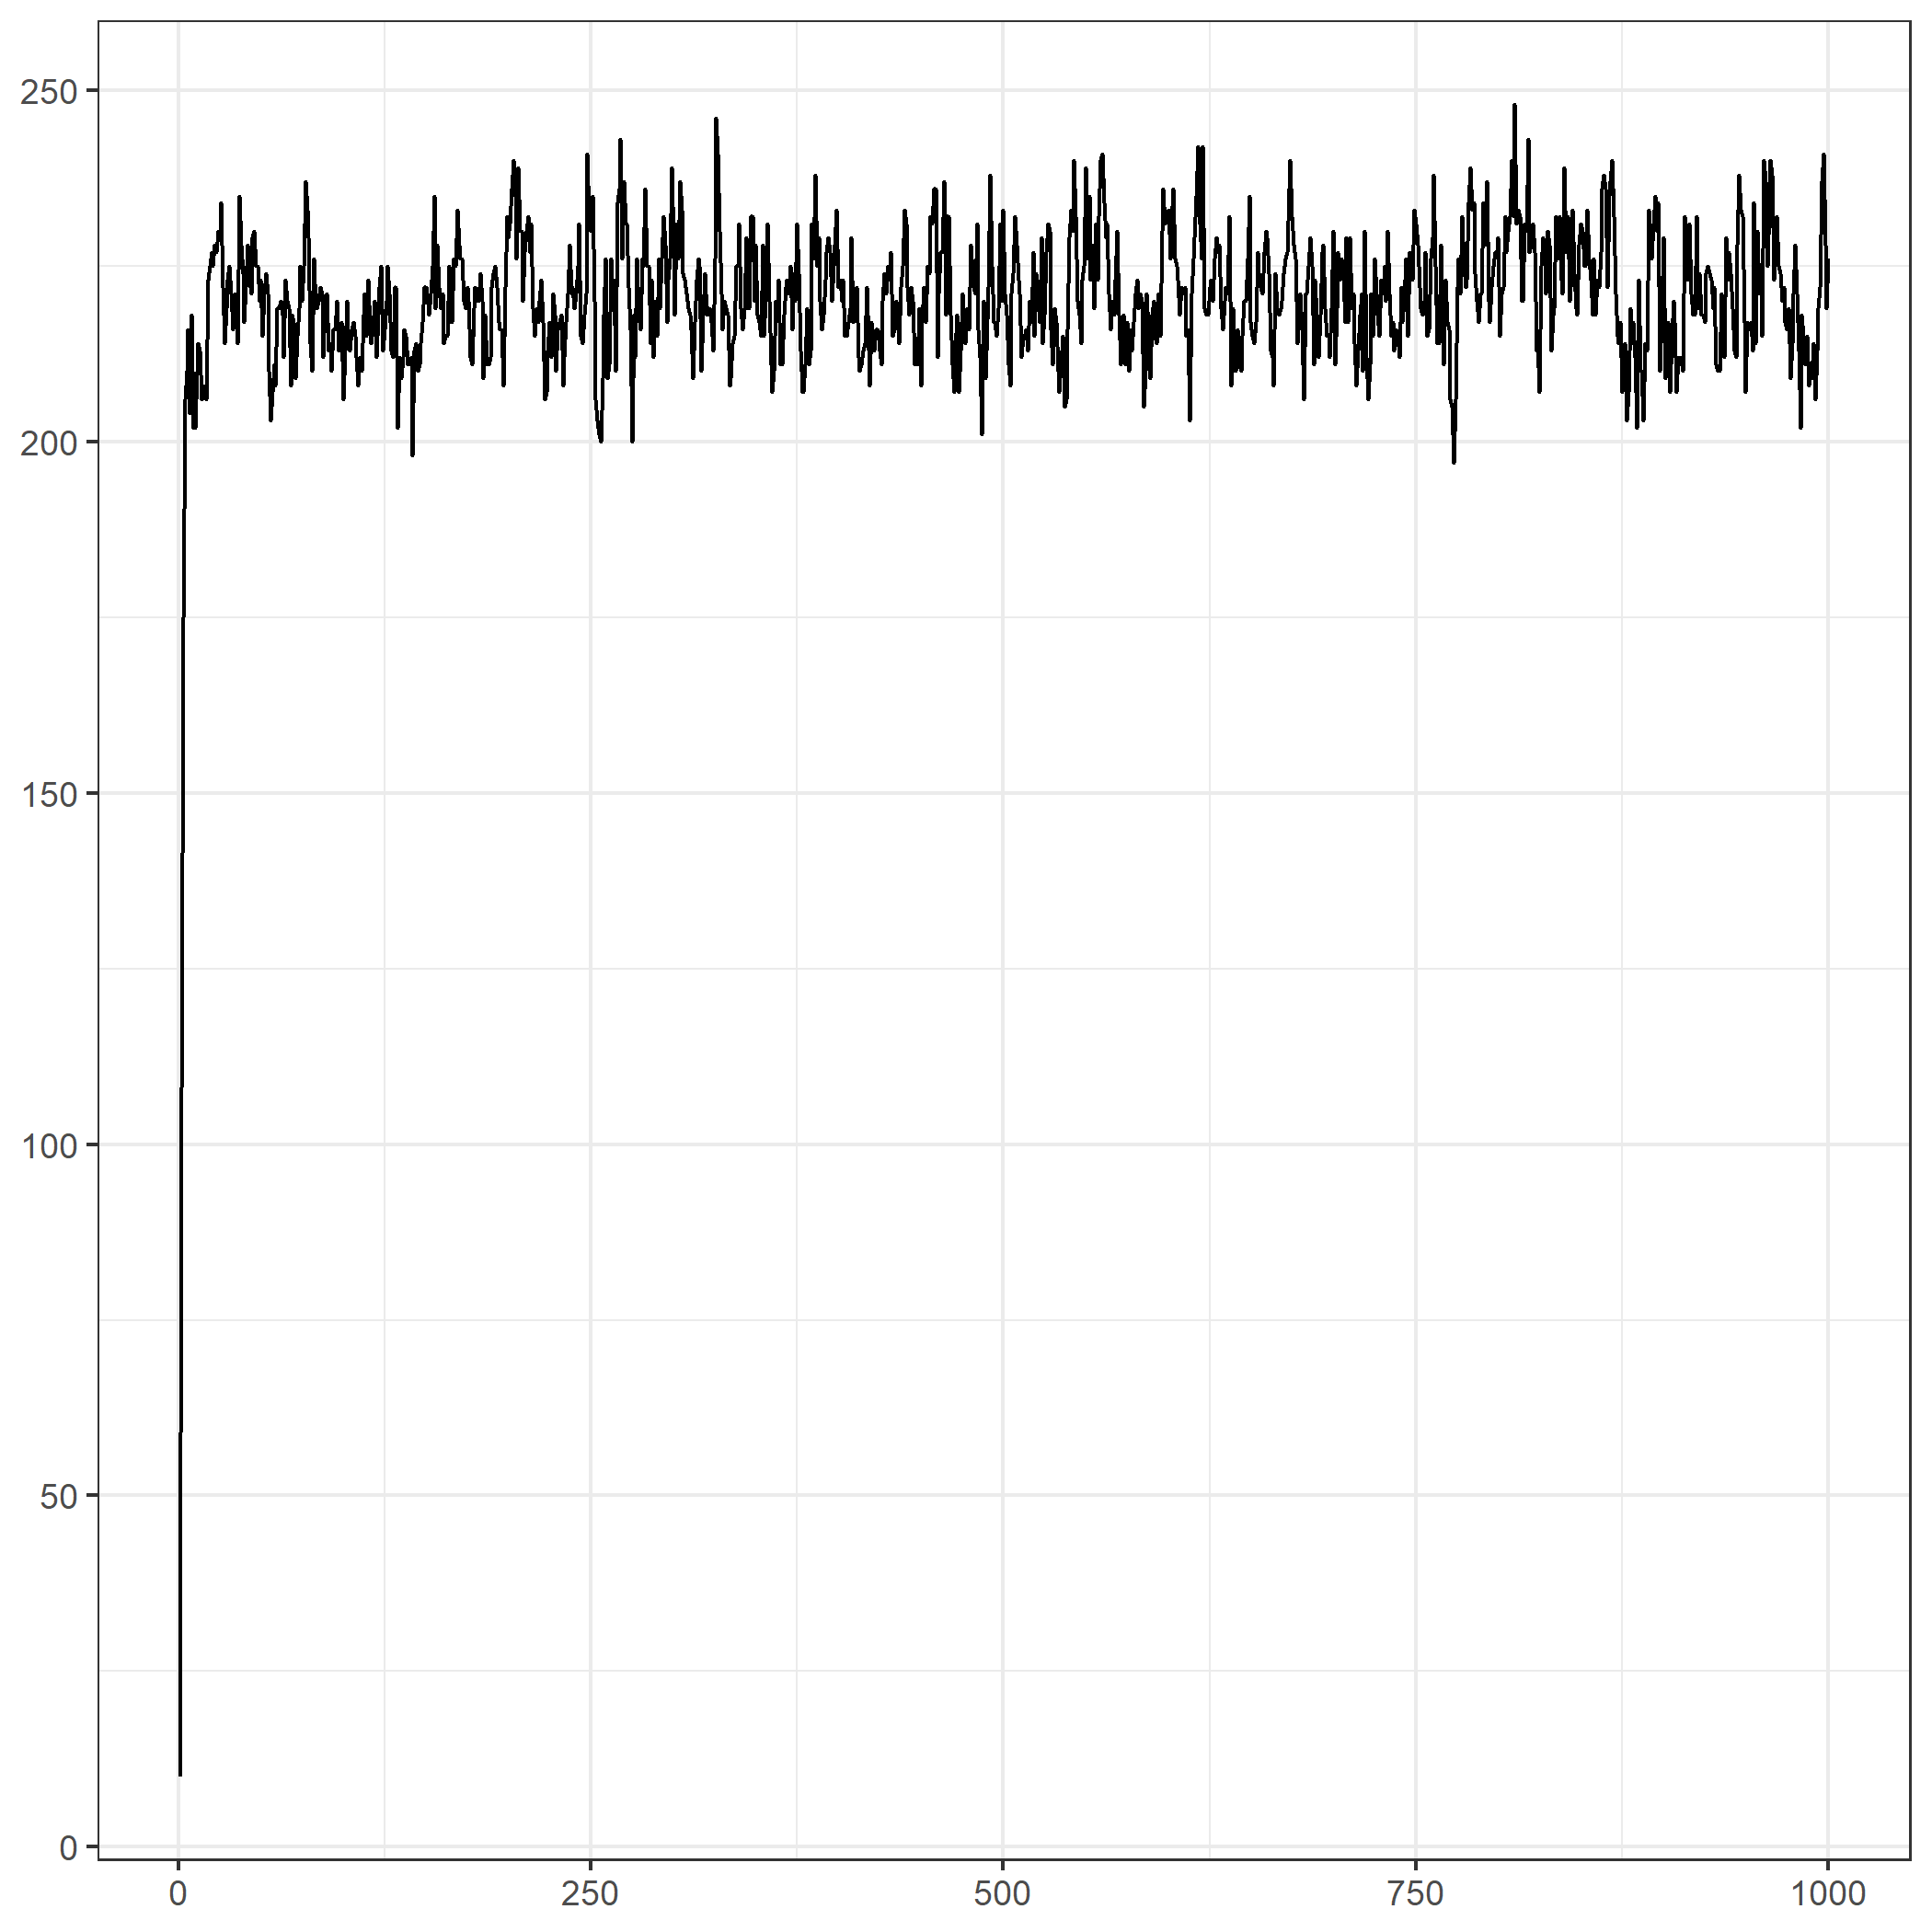
\includegraphics[width=0.6\textwidth]{../notes/figures/el_salvador/overlap_trace} 
		
	}
	
	\caption{Traceplot for number of matches found across datasets in El Salvador case study}\label{fig:overlap_trace}
\end{figure}

\begin{figure}[t]
	
	{\centering 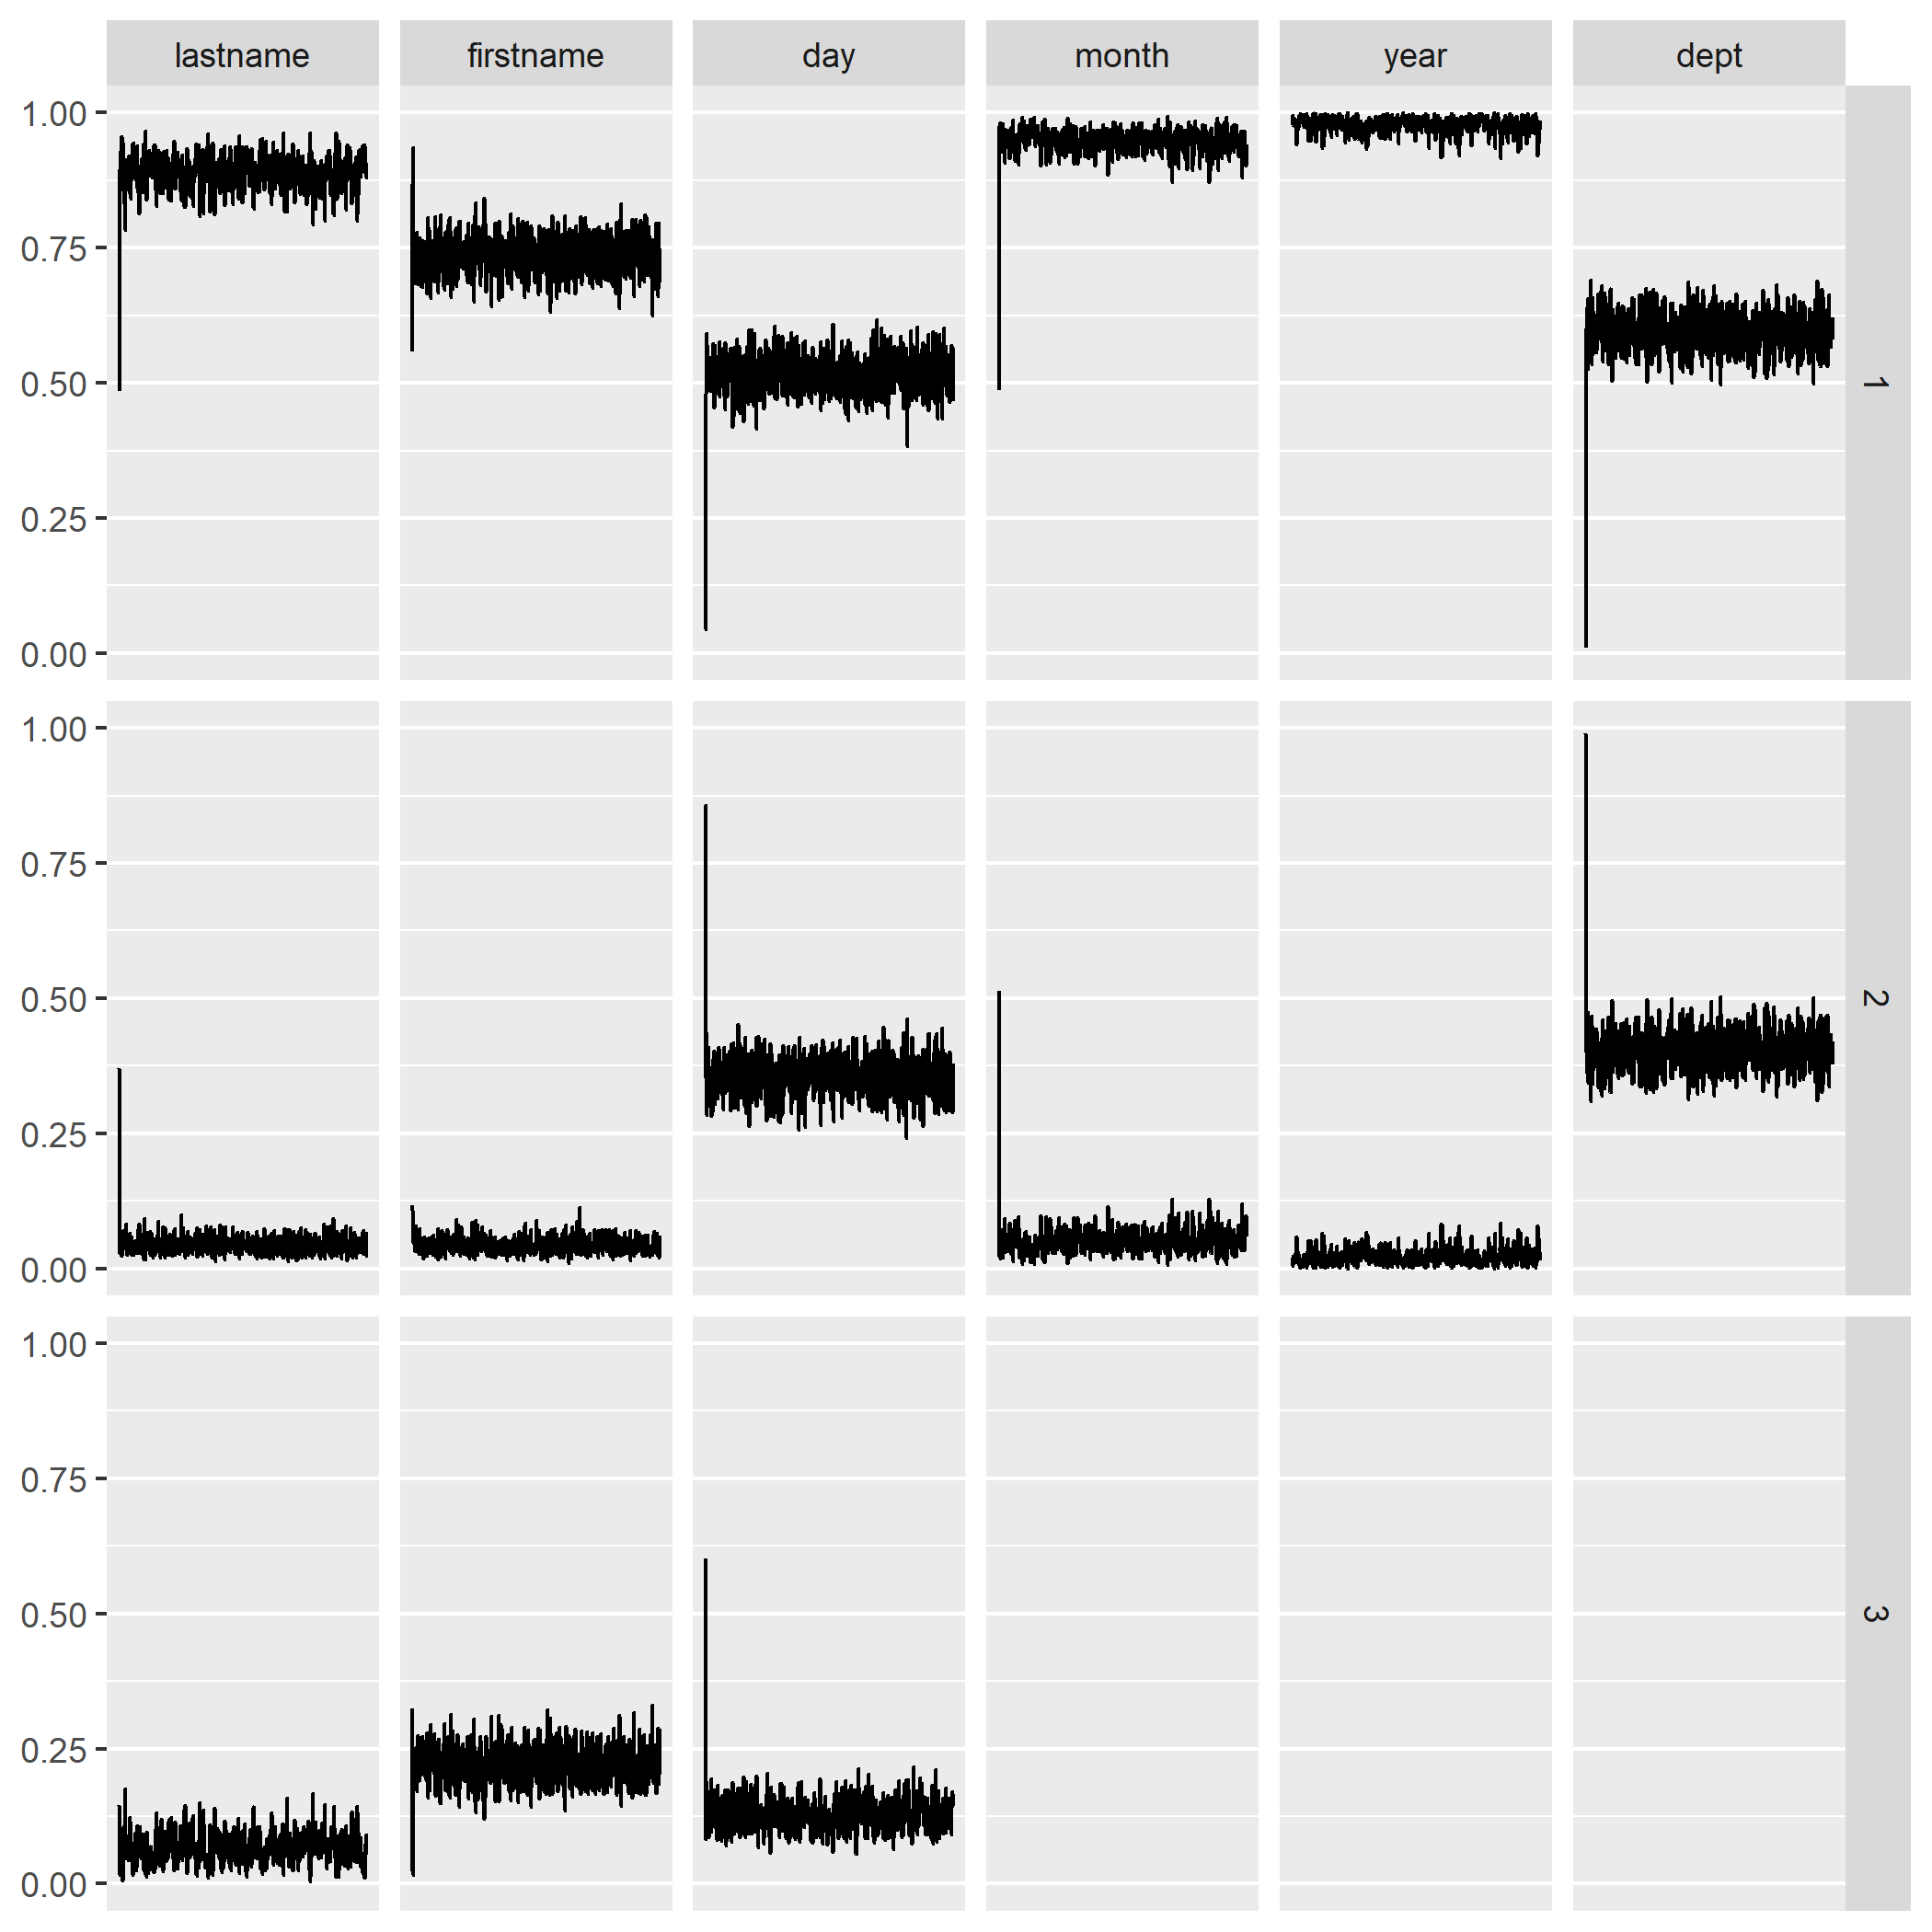
\includegraphics[width=0.6\textwidth]{../notes/figures/el_salvador/m_trace} 
		
	}
	
	\caption{Traceplot for m parameter in El Salvador case study}\label{fig:m_trace}
\end{figure}

\begin{figure}[t]
	
	{\centering 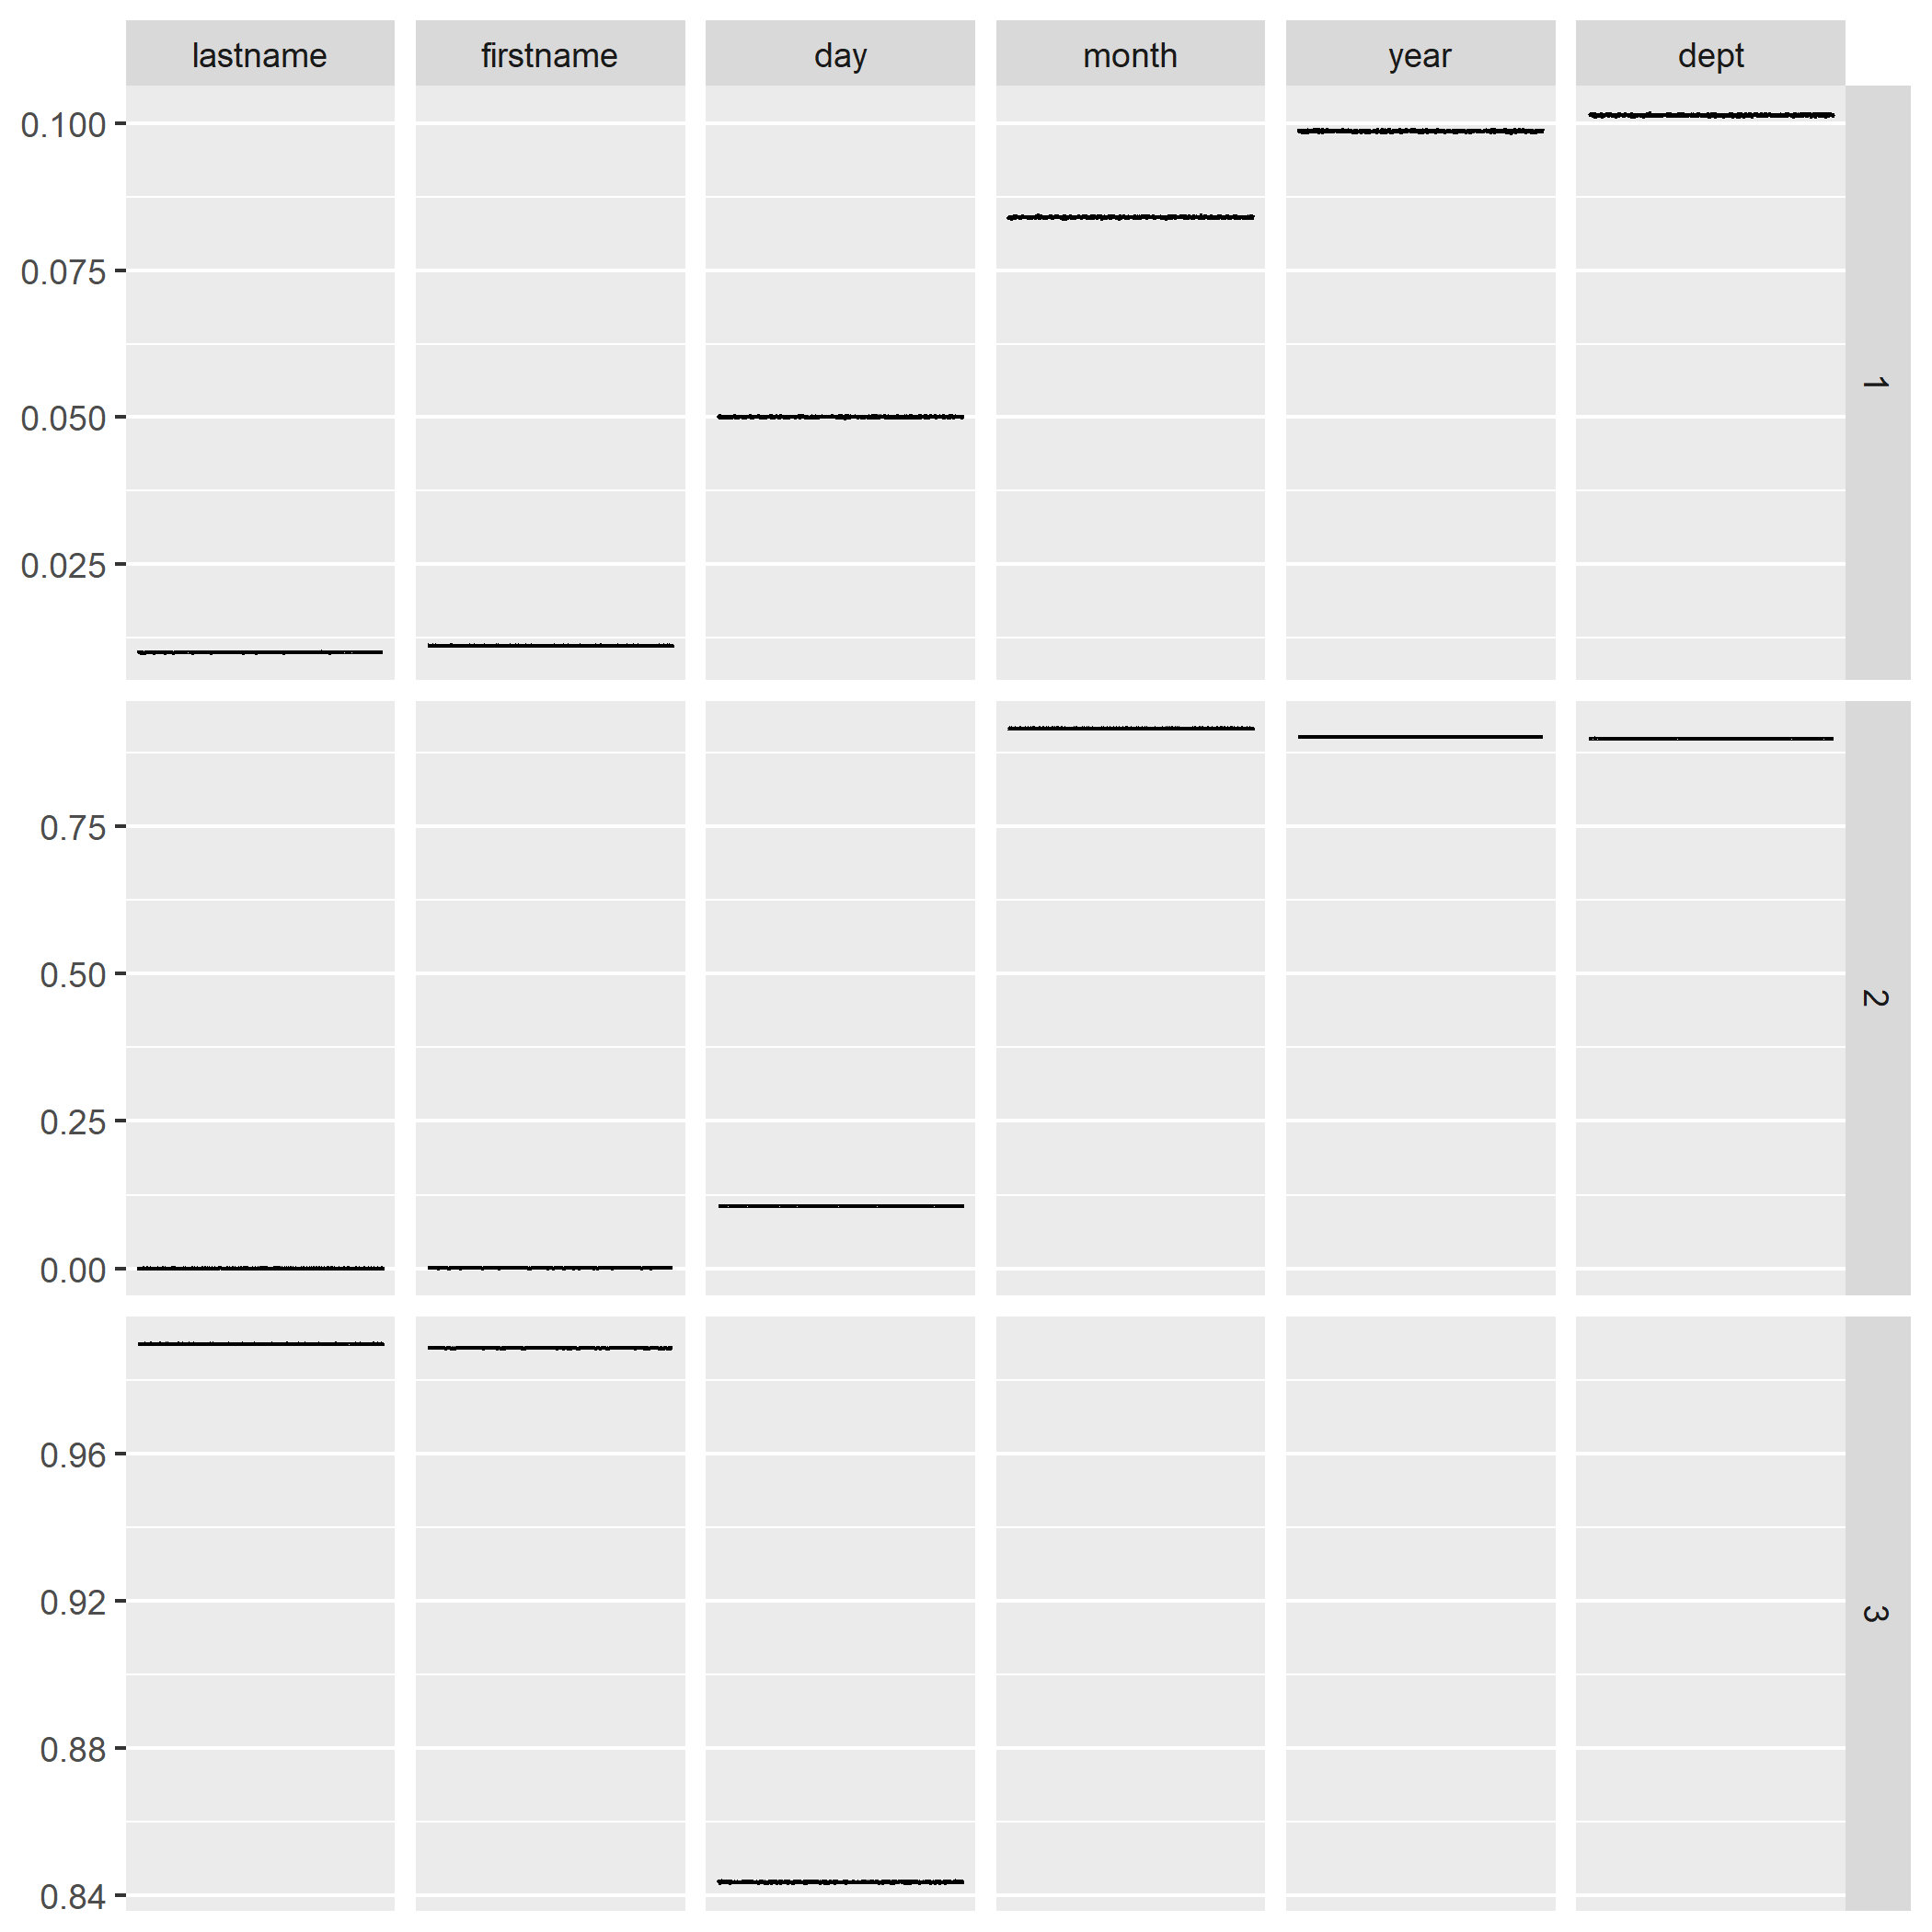
\includegraphics[width=0.6\textwidth]{../notes/figures/el_salvador/u_trace} 
		
	}
	
	\caption{Traceplot for u parameter in El Salvador case study}\label{fig:u_trace}
\end{figure}

\bigskip

\bibliographystyle{jasa}
{
\footnotesize
\bibliography{biblio}
}

\end{document}
